\RequirePackage[l2tabu, orthodox]{nag}
\documentclass[10pt]{scrartcl}
% \documentclass[10pt]{article}
\usepackage[T1]{fontenc}
\usepackage{amsmath,amsfonts,amssymb}
\usepackage{mathtools}
\usepackage{color,soul}
\usepackage{fullpage}
\usepackage{enumerate}
\usepackage{graphicx}
\usepackage[colorlinks=true,urlcolor=blue]{hyperref}
% \usepackage[justification=center]{caption}
\usepackage{subcaption}
\usepackage{deluxetable}
\usepackage{verbatim}
\usepackage{fancyvrb}
\usepackage{listings}
\usepackage[activate={true,nocompatibility},final,tracking=true,kerning=true,spacing=true,factor=1100,stretch=10,shrink=10]{microtype}

\lstset{%
language=C++,                   % choose the language of the code
basicstyle=\footnotesize\sffamily,%\ttfamily\footnotesize,       % the size of the fonts that are used for the code
numbers=left,                   % where to put the line-numbers
numberstyle=\footnotesize,      % the size of the fonts that are used for the line-numbers
stepnumber=1,                   % the step between two line-numbers. If it is 1 each line will be numbered
numbersep=5pt,                  % how far the line-numbers are from the code
showspaces=false,               % show spaces adding particular underscores
showstringspaces=false,         % underline spaces within strings
showtabs=false,                 % show tabs within strings adding particular underscores
% frame=single,                   % adds a frame around the code
backgroundcolor=\color{Light},
columns=fullflexible,
tabsize=2,                      % sets default tabsize to 2 spaces
captionpos=b,                   % sets the caption-position to bottom
breaklines=true,                % sets automatic line breaking
breakatwhitespace=false,        % sets if automatic breaks should only happen at whitespace
escapeinside={\%*}{*)}          % if you want to add a comment within your code
}


\definecolor{Light}{gray}{.90}
\sethlcolor{Light}


\title{Using 1D Sums to Find Fiducials}
\author{Jeren Suzuki}
\date{Last Edited \today}

\begin{document}

\maketitle
\pagenumbering{Roman}
\tableofcontents
\clearpage
\pagenumbering{arabic}

\section{Introduction} % (fold)
\label{sec:introduction}
Instead of using convolution filters, we look at 1D sums to identify fiducials. 
% section introduction (end)

\begin{figure}[!ht]
    \begin{subfigure}[b]{.5\linewidth}
        \centering
        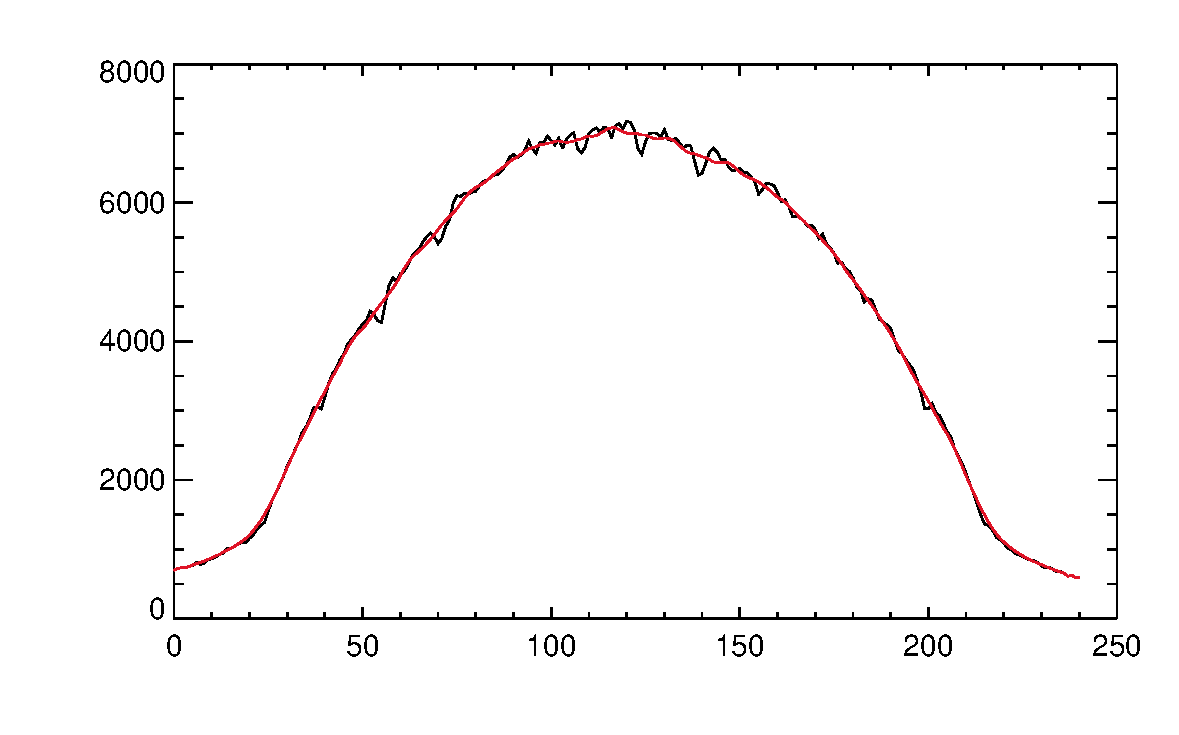
\includegraphics[width=\linewidth]{../plots_tables_images/smooth_expl.eps}
        \caption{This is the 1D sum of a solar image. Small dips are seen in the profile corresponding to fiducials. The line in red is the sum smoothed by 10 pixels.}
    \end{subfigure}
    \begin{subfigure}[b]{.5\linewidth}
        \centering
        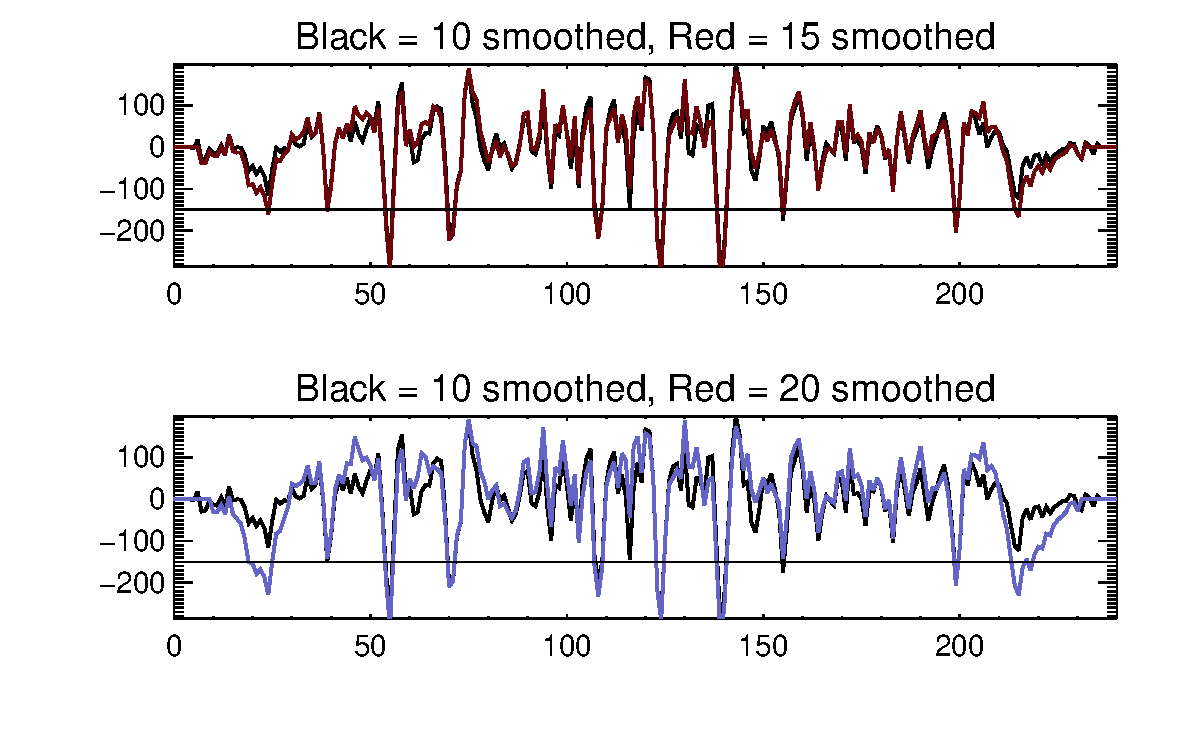
\includegraphics[width=\linewidth]{../plots_tables_images/smoothcomp.eps}
        \caption{We subtract the smoothed profile from the raw data to emphasize dips. Comparisons of the smooth amount change the width and number of the dips, although not really the depth.}
        \label{threshed}
    \end{subfigure}
    \caption{}
    \label{smoothed}
\end{figure}

\section{Finding Fiducials} % (fold)
\label{sec:finding_fiducials}

For each position below a certain threshold (see Figure \ref{threshed}) a row/column  is returned. Once we have an array of possible fiducial row and column positions, they are matched against each other using a method that iteratively checks to see if a pair of coordinates is a fiducial. For Figure \ref{smoothtest}, the white squares are pairs where both X and Y coordinates were returned from thresholding, the yellow squares are pairs where one of the coordinates had to be guessed since it was not found.

% \begin{figure}[!ht]
   
    % \includegraphics[width=\linewidth]{../plots_tables_images/morefid.eps}
    % \caption{The white squares are pairs where both X and Y coordinates were returned from thresholding, the yellow squares are pairs where one of the coordinates had to be guessed since it was not found.}
    % \label{smoothed}
% \end{figure}

\begin{figure}[!ht]
    \hspace{-1.0in}
    \begin{subfigure}[b]{.75\linewidth}
        \centering
        \includegraphics[width=\linewidth]{../plots_tables_images/morefid.eps}
        \caption{10 pixel smoothed sum}
    \end{subfigure}
    \hspace{-1.0in}
    \begin{subfigure}[b]{.75\linewidth}
        \centering
        \includegraphics[width=\linewidth]{../plots_tables_images/lessfid.eps}
        \caption{20 pixel smoothed sum}
    \end{subfigure}
    \caption{}
    \label{smoothtest}
\end{figure}


There is a problem with the row/columns returned from thresholding the sum - smoothed sum; sometimes the number of indices don't match up. i.e., we ``see'' 7 fiducials in one axis but only 5 in another. How do we correctly rule out extra fiducials in one axis but not the other?

Also, this summing implementation aims to simplify and speed up the fiducial finding process, but once we have an array of X and Y positions of fiducials, verifying they actually lie on fiducials requires methods we tried to move away from. 

\subsection{Using Gaussian Fits} % (fold)
\label{sub:using_gaussian_fits}
    It turns out that using Gaussian fits to find fiducials is faster than expected. After finding all possible row/column combinations of fiducials, each candidate's 1D sum is fitted with a Gaussian, regardless of being a fiducial or not. We look at the $\chi^2/N$ statistic to order out fits by how `fiducial' they are. Since we only need, say, $M$ fiducials, we can sort the fiducials by their $\chi^2/N$ and pick the top 5.\\

\begin{figure}
    \centering
    \includegraphics[width=\linewidth]{../plots_tables_images/gfitted.eps}
    \caption{Gaussian fits with a $\chi^2/N > 20$}
\end{figure}

\begin{figure}
    \centering
    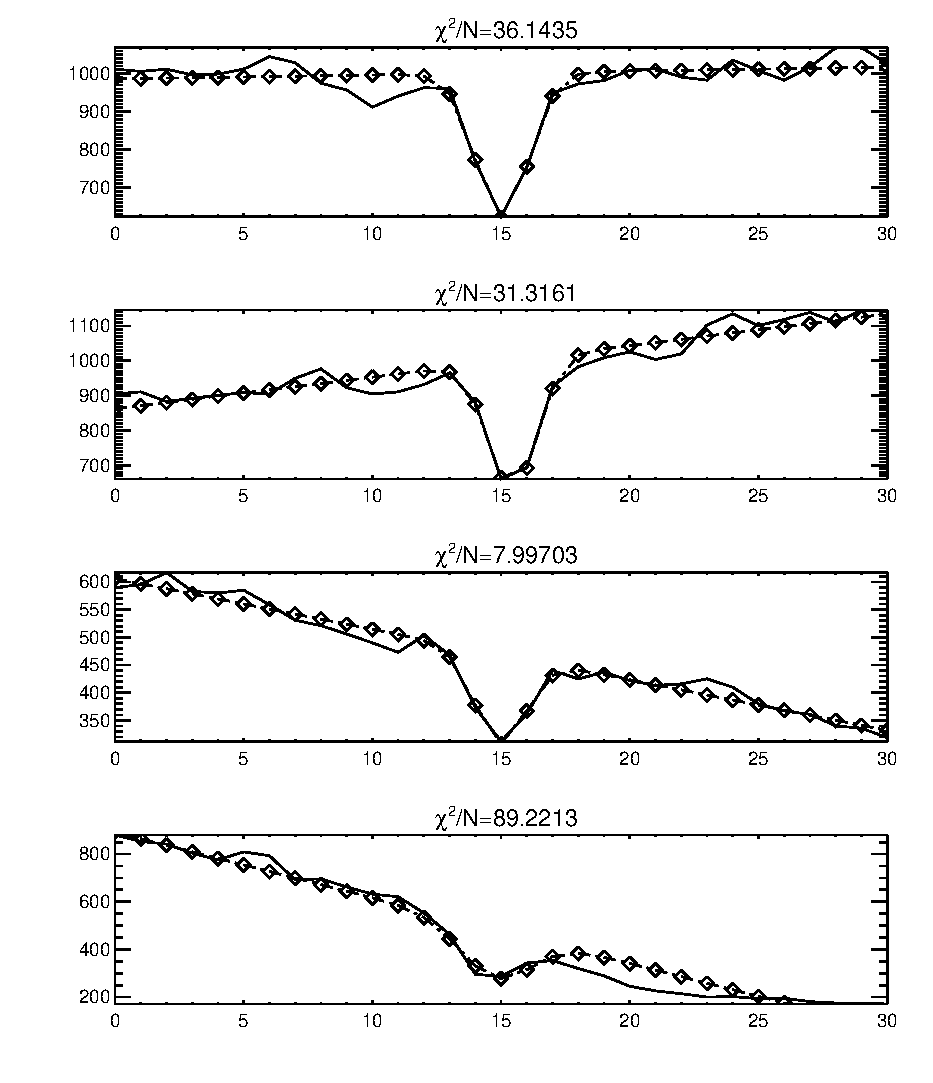
\includegraphics[width=\linewidth]{../plots_tables_images/gaussfitcomp.eps}
    \caption{These are all real fiducials, ranging from looking nice (first two) to being on the solar limb (last 2).}
\end{figure}

We're walking a fine line here; instead of minimizing our $\chi^2/N$, we're maximizing it.

% \begin{figure}[!ht]
%
%     \hspace{-1.0in}
%     \begin{subfigure}[b]{.5\linewidth}
%         \centering
%         \includegraphics[width=\linewidth]{../plots_tables_images/gfitted.eps}
%         \caption{Gaussian fits with a $\chi^2/N > 20$}
%     \end{subfigure}
%     \hspace{-1.0in}
%     \begin{subfigure}[b]{.8\linewidth}
%         \centering
%         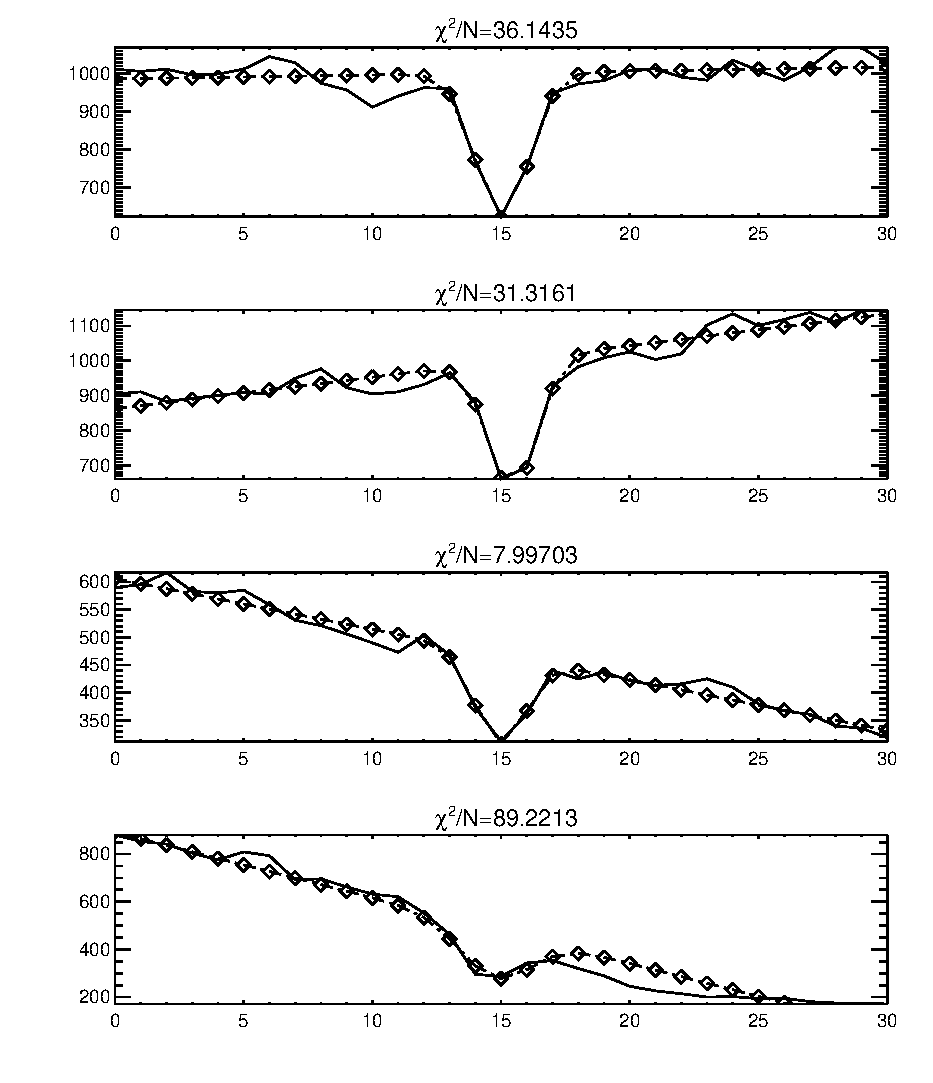
\includegraphics[width=\linewidth]{../plots_tables_images/gaussfitcomp.eps}
%         \caption{These are all real fiducials, ranging from looking nice (first two) to being on the solar limb (last 2). Not sure why the third $\chi^2/N$ is so low...}
%     \end{subfigure}
%     \caption{}
%     \label{smoothed}
% \end{figure}

%Can't include this because of time needed for subpix fitting
% \subsubsection{Time Spent} % (fold)
% \label{sub:time_spent}

% The program takes approximately .009 seconds, compared to \hl{\texttt{fid\_faster()}}'s .014 seconds and \hl{\texttt{fid\_locate}}'s .06 seconds. \hl{\texttt{fid\_faster()}} used two 1D convolution filters and looked for local minima, \hl{\texttt{fid\_locate()}} used a single 2D convolution filter and looked for local minima.

% % subsection time_spent (end)

% subsection using_gaussian_fits (end)

\subsection{1D Sums} % (fold)
\label{sub:1d_sums}
1D Gaussians provide a robust method to identify fiducials but they take quite a long time to run. An alternative is to use another 1D sum to identify fiducial shapes in cropped areas defined by running a larger 1D filter. Figures \ref{lotsofcrop} and \ref{lotsofplot} illustrate the relationship between the region we look at versus what the 1D sums look like. In Figure \ref{1dsumsarethebest}, 7 fiducials are found using the 1D sum method.

\begin{figure}
    \centering
    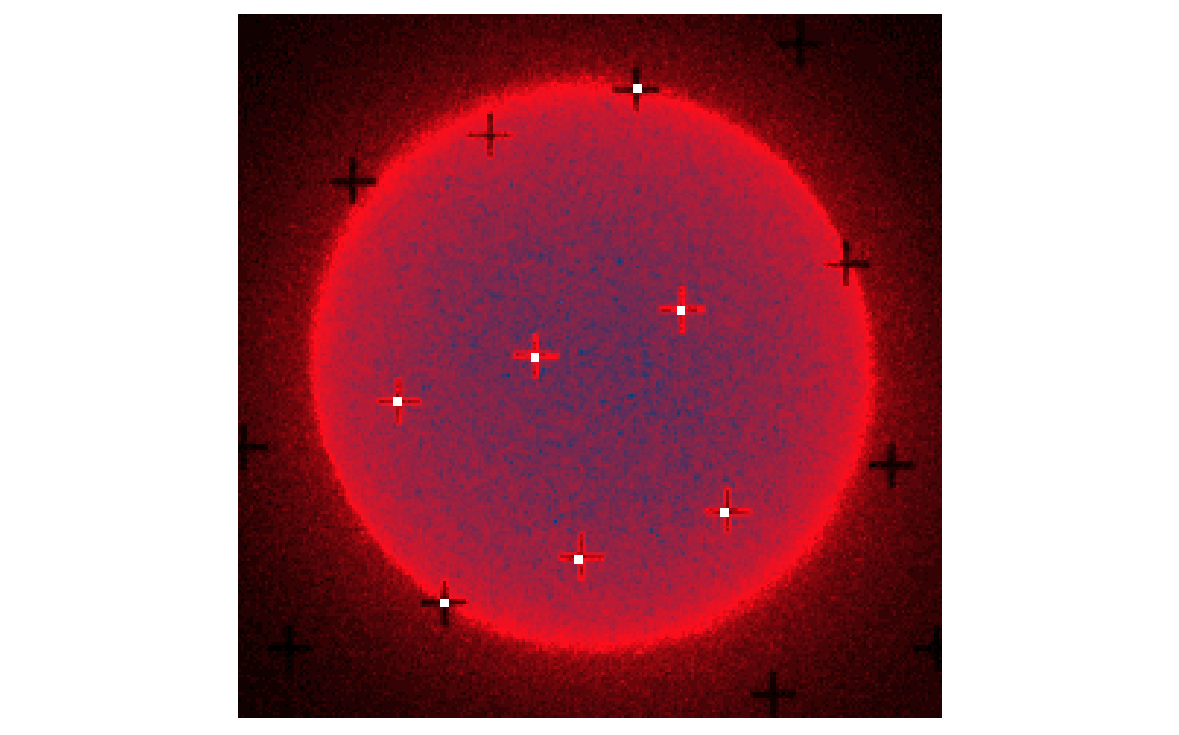
\includegraphics[width=\linewidth]{../plots_tables_images/1dsums.eps}
    \caption{Fiducials found using a 1D summing method on the entire image followed by another 1D summing method on a cropped region based on fiducial candidates. Using a threshold of 100 on an \hl{\texttt{smooth(array,10) - array}} identifies the white squares.}
    \label{1dsumsarethebest}
\end{figure}

\begin{figure}[!ht]
    \vspace{-0.5in}
    \begin{subfigure}[b]{.3\linewidth}
        \centering
        \includegraphics[width=1.2\linewidth]{../plots_tables_images/1d1dcrop_0_0.eps}
        % \caption{}
    \end{subfigure}
    \begin{subfigure}[b]{.3\linewidth}
        \centering
        \includegraphics[width=1.2\linewidth]{../plots_tables_images/1d1dcrop_0_1.eps}
        % \caption{}
    \end{subfigure}
    % \hspace{-1.0in}
    \begin{subfigure}[b]{.3\linewidth}
        \centering
        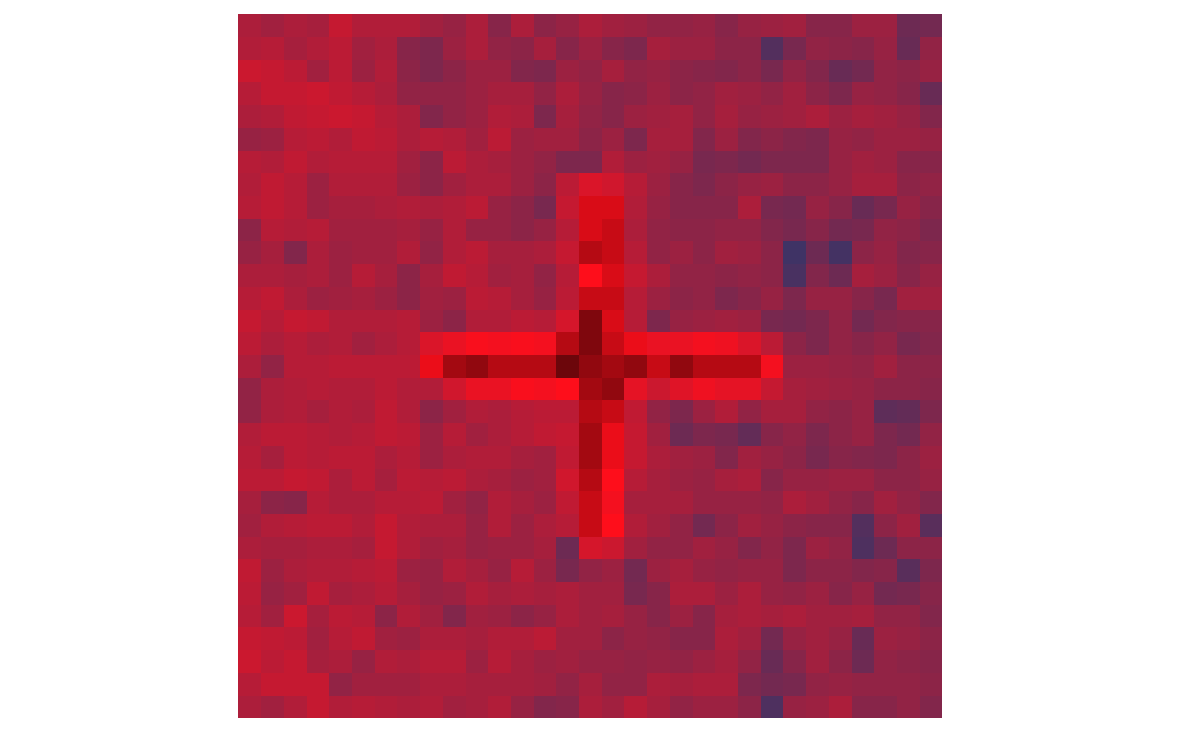
\includegraphics[width=1.2\linewidth]{../plots_tables_images/1d1dcrop_0_4.eps}
        % \caption{}
    \end{subfigure}

    \begin{subfigure}[b]{.3\linewidth}
        \centering
        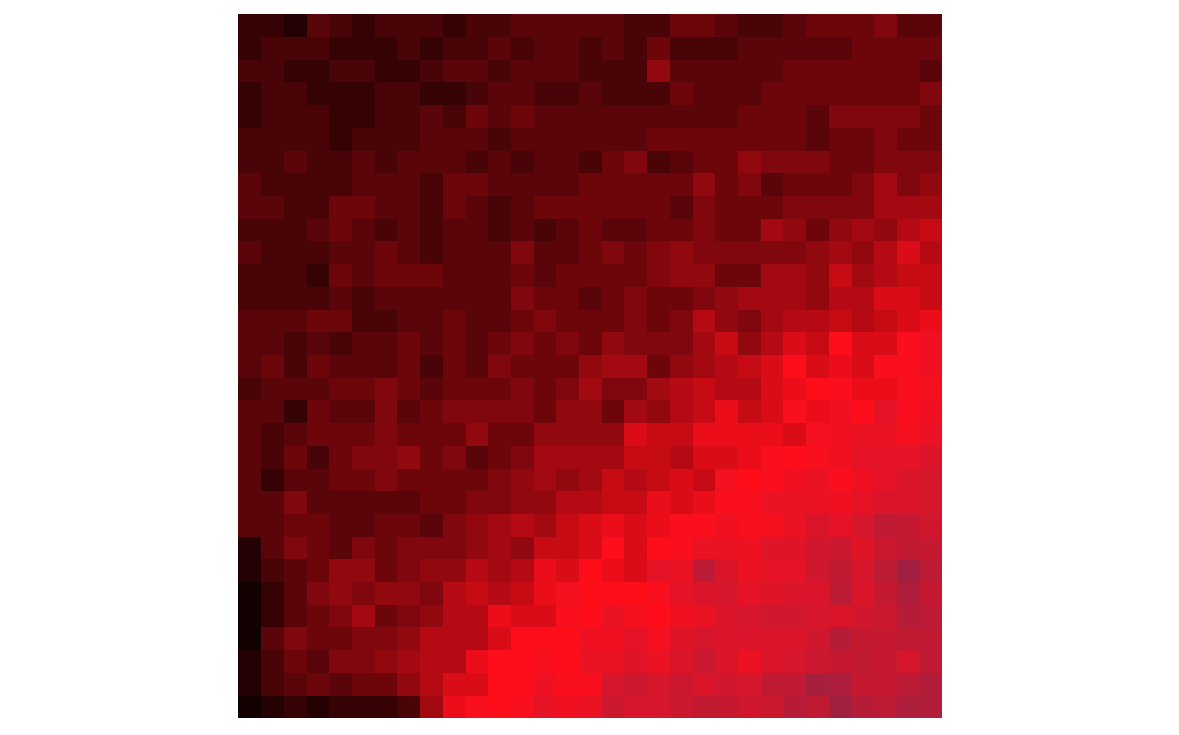
\includegraphics[width=1.2\linewidth]{../plots_tables_images/1d1dcrop_0_8.eps}
        % \caption{}
    \end{subfigure}
    \begin{subfigure}[b]{.3\linewidth}
        \centering
        \includegraphics[width=1.2\linewidth]{../plots_tables_images/1d1dcrop_0_9.eps}
        % \caption{}
    \end{subfigure}
    % \hspace{-1.0in}
    \begin{subfigure}[b]{.3\linewidth}
        \centering
        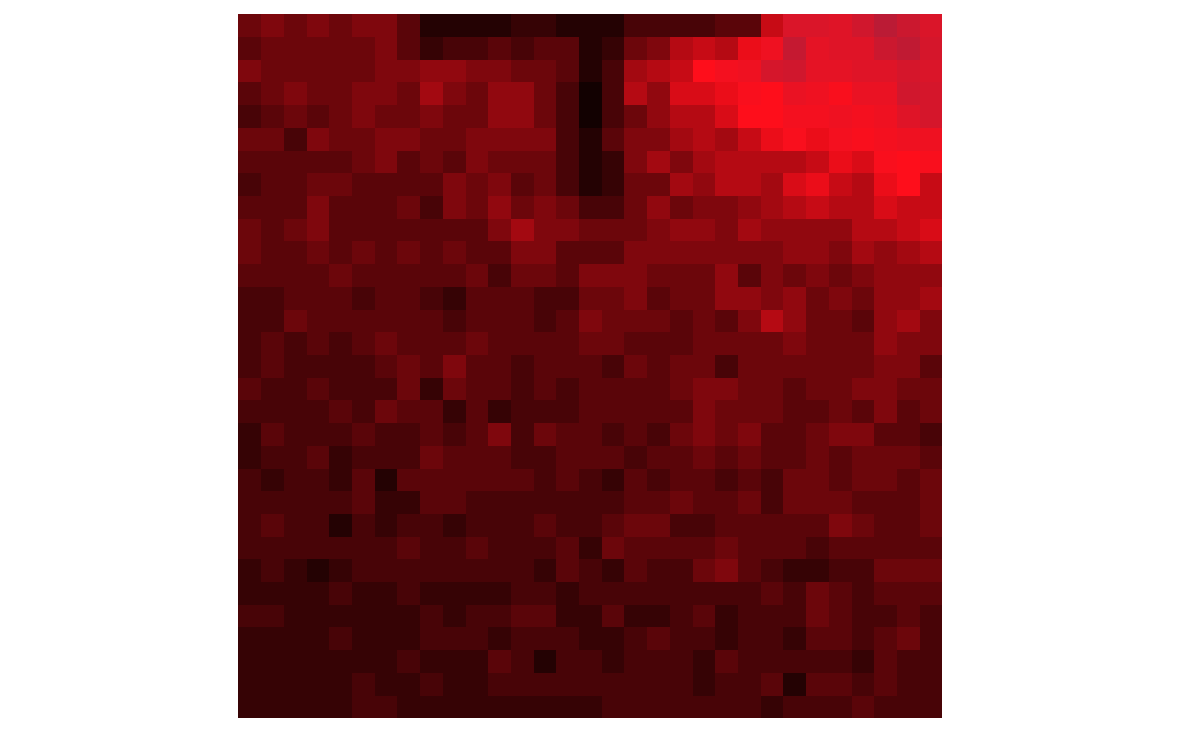
\includegraphics[width=1.2\linewidth]{../plots_tables_images/1d1dcrop_1_0.eps}
        % \caption{}
    \end{subfigure}


    \begin{subfigure}[b]{.3\linewidth}
        \centering
        \includegraphics[width=1.2\linewidth]{../plots_tables_images/1d1dcrop_1_1.eps}
        % \caption{}
    \end{subfigure}
    \begin{subfigure}[b]{.3\linewidth}
        \centering
        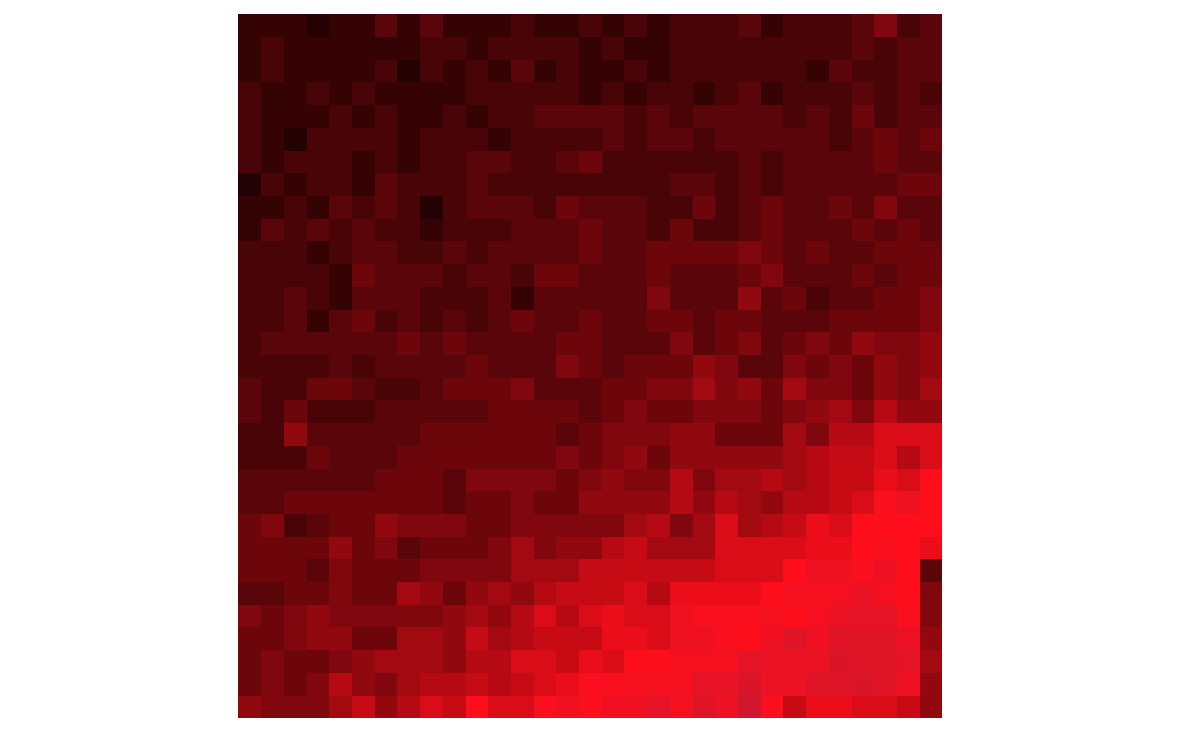
\includegraphics[width=1.2\linewidth]{../plots_tables_images/1d1dcrop_1_9.eps}
        % \caption{}
    \end{subfigure}
    % \hspace{-1.0in}
    \begin{subfigure}[b]{.3\linewidth}
        \centering
        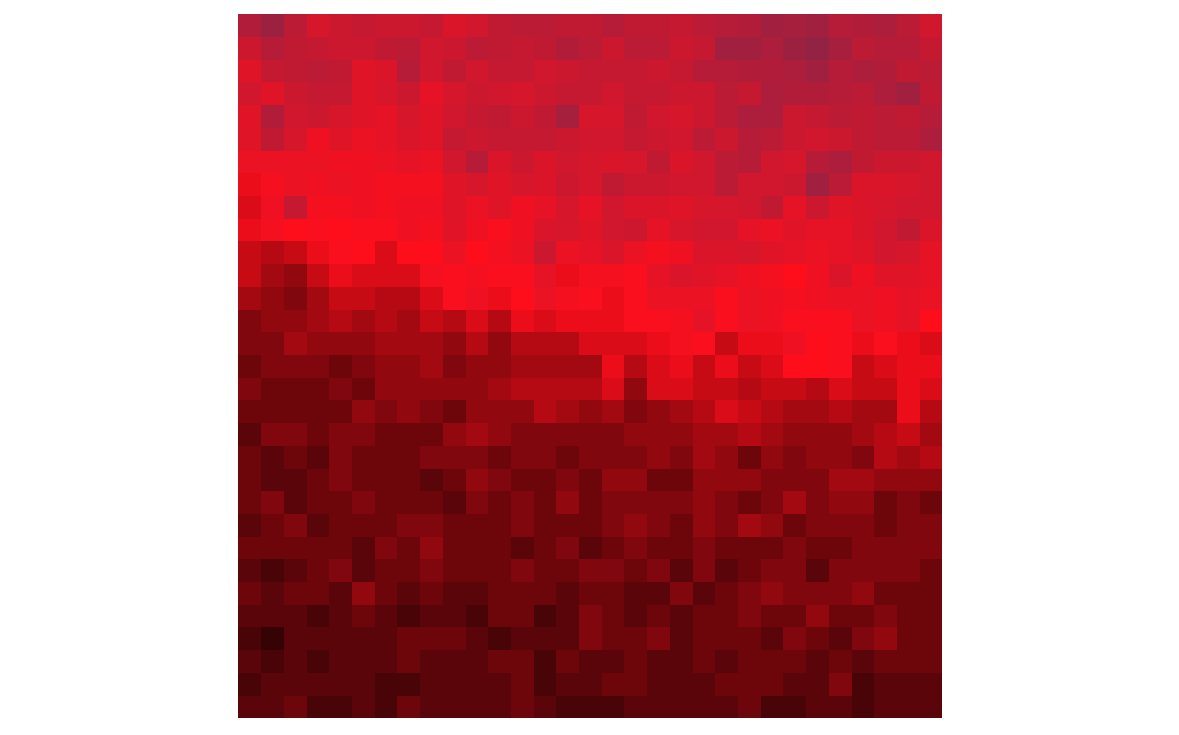
\includegraphics[width=1.2\linewidth]{../plots_tables_images/1d1dcrop_2_0.eps}
        % \caption{}
    \end{subfigure}


    \begin{subfigure}[b]{.3\linewidth}
        \centering
        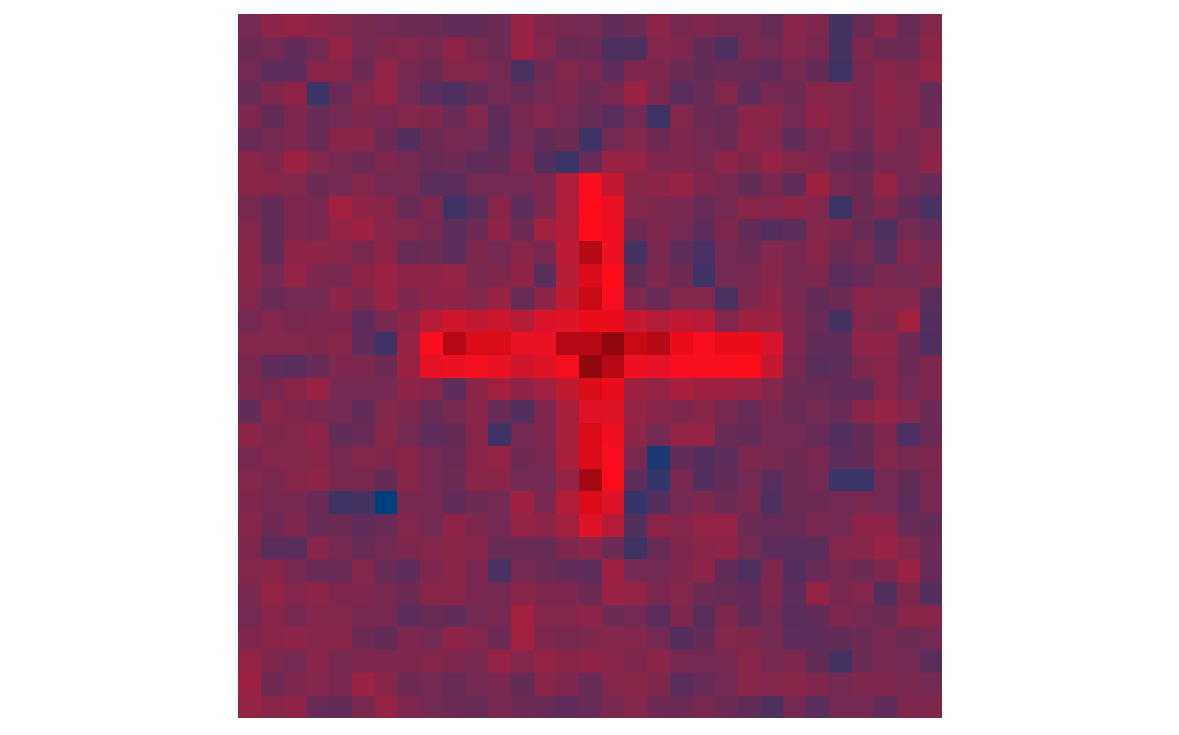
\includegraphics[width=1.2\linewidth]{../plots_tables_images/1d1dcrop_2_5.eps}
        % \caption{}
    \end{subfigure}
    \begin{subfigure}[b]{.3\linewidth}
        \centering
        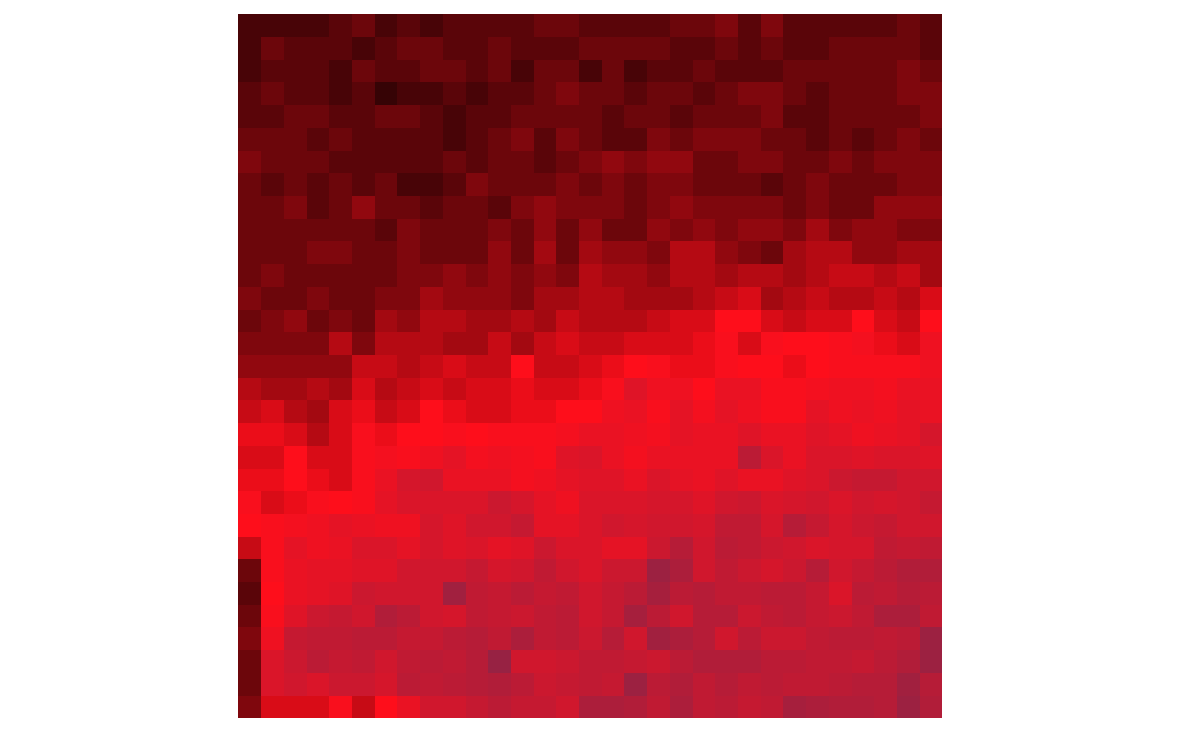
\includegraphics[width=1.2\linewidth]{../plots_tables_images/1d1dcrop_2_9.eps}
        % \caption{}
    \end{subfigure}
    % \hspace{-1.0in}
    \begin{subfigure}[b]{.3\linewidth}
        \centering
        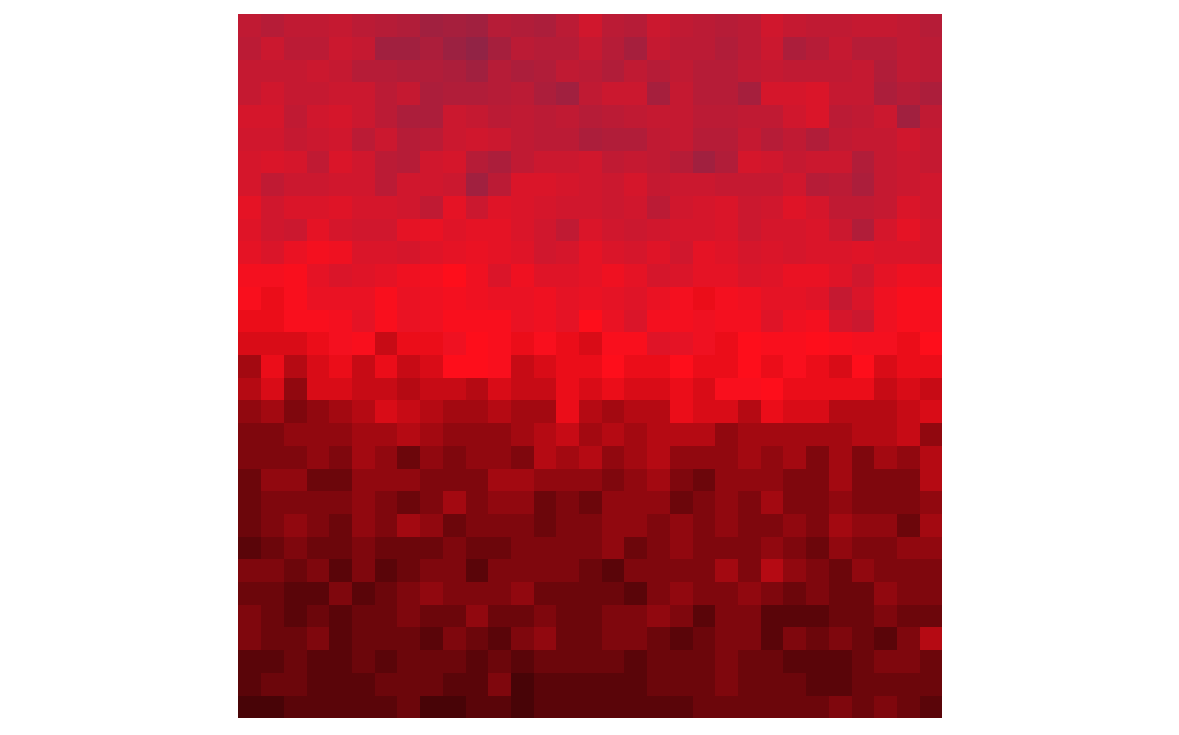
\includegraphics[width=1.2\linewidth]{../plots_tables_images/1d1dcrop_3_0.eps}
        % \caption{}
    \end{subfigure}


    \begin{subfigure}[b]{.3\linewidth}
        \centering
        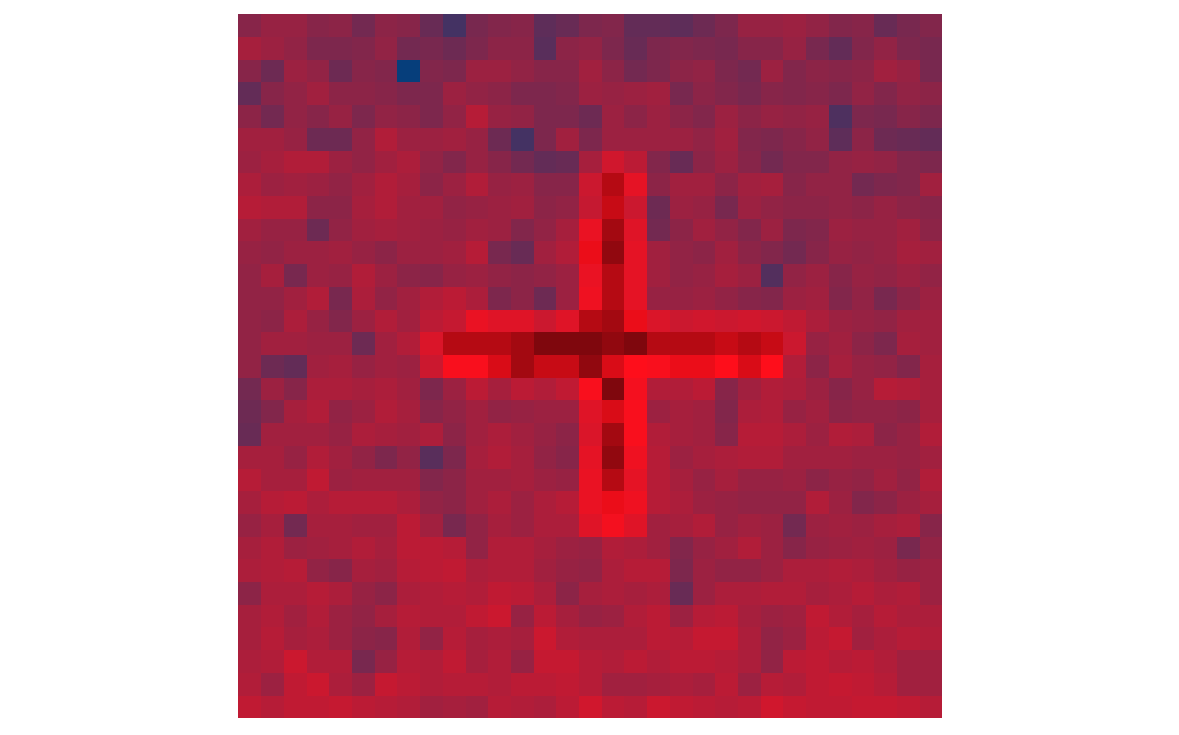
\includegraphics[width=1.2\linewidth]{../plots_tables_images/1d1dcrop_3_2.eps}
        % \caption{}
    \end{subfigure}
    \begin{subfigure}[b]{.3\linewidth}
        \centering
        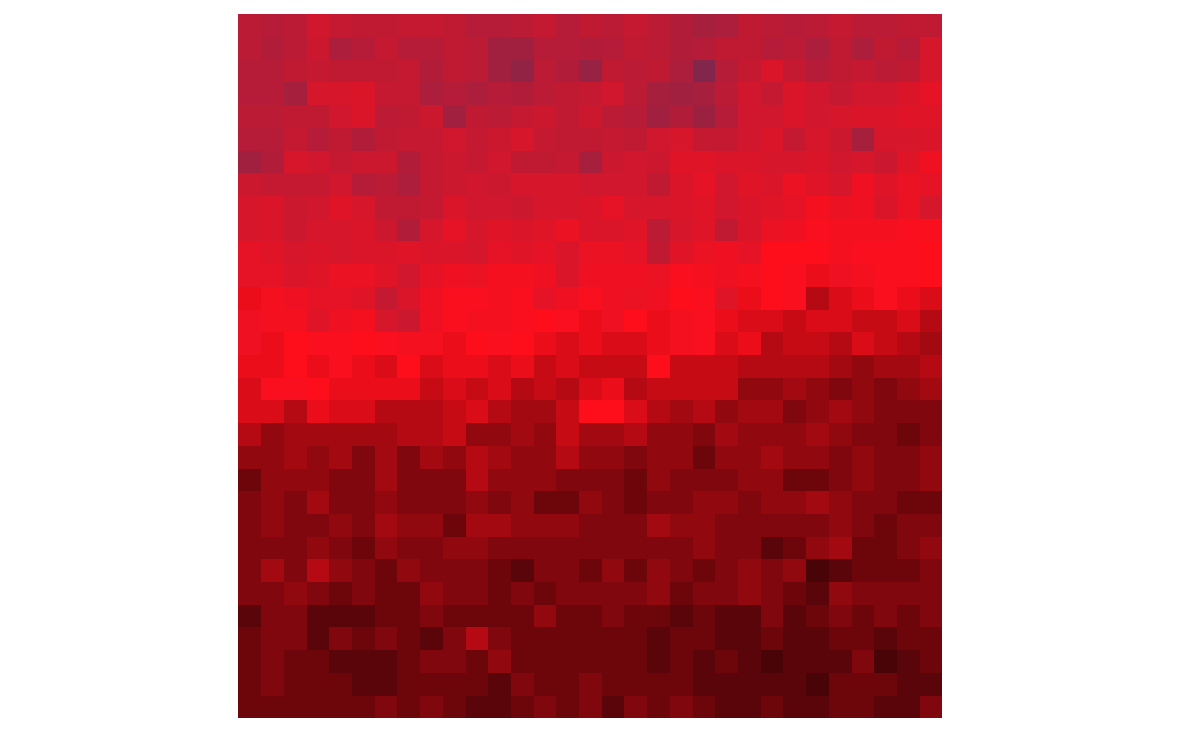
\includegraphics[width=1.2\linewidth]{../plots_tables_images/1d1dcrop_4_0.eps}
        % \caption{}
    \end{subfigure}
    % \hspace{-1.0in}
    \begin{subfigure}[b]{.3\linewidth}
        \centering
        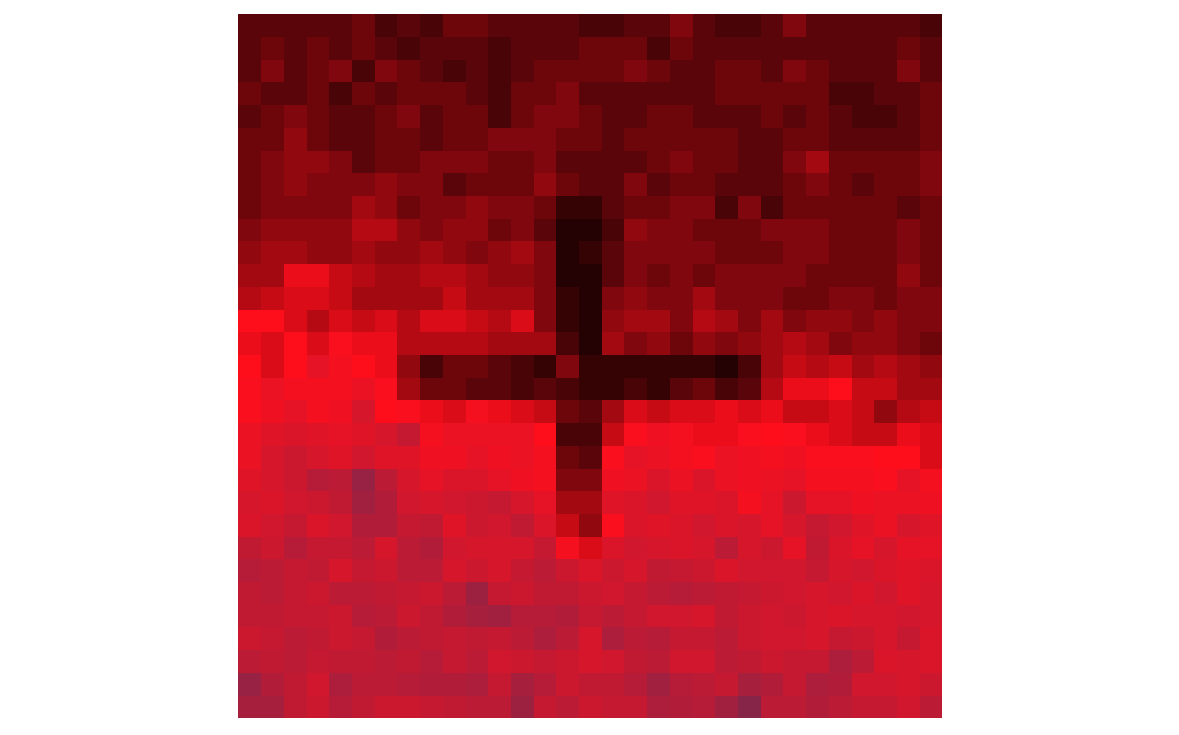
\includegraphics[width=1.2\linewidth]{../plots_tables_images/1d1dcrop_4_9.eps}
        % \caption{}
    \end{subfigure}


    \begin{subfigure}[b]{.3\linewidth}
        \centering
        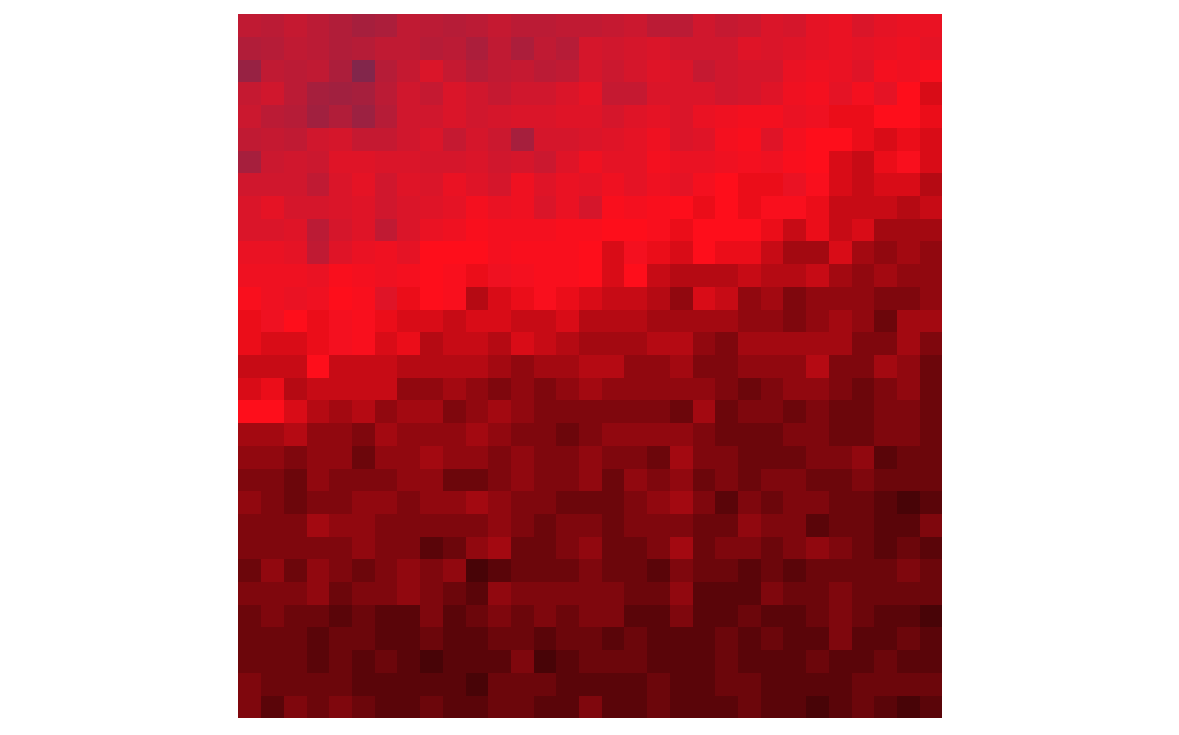
\includegraphics[width=1.2\linewidth]{../plots_tables_images/1d1dcrop_5_0.eps}
        % \caption{}
    \end{subfigure}
    \begin{subfigure}[b]{.3\linewidth}
        \centering
        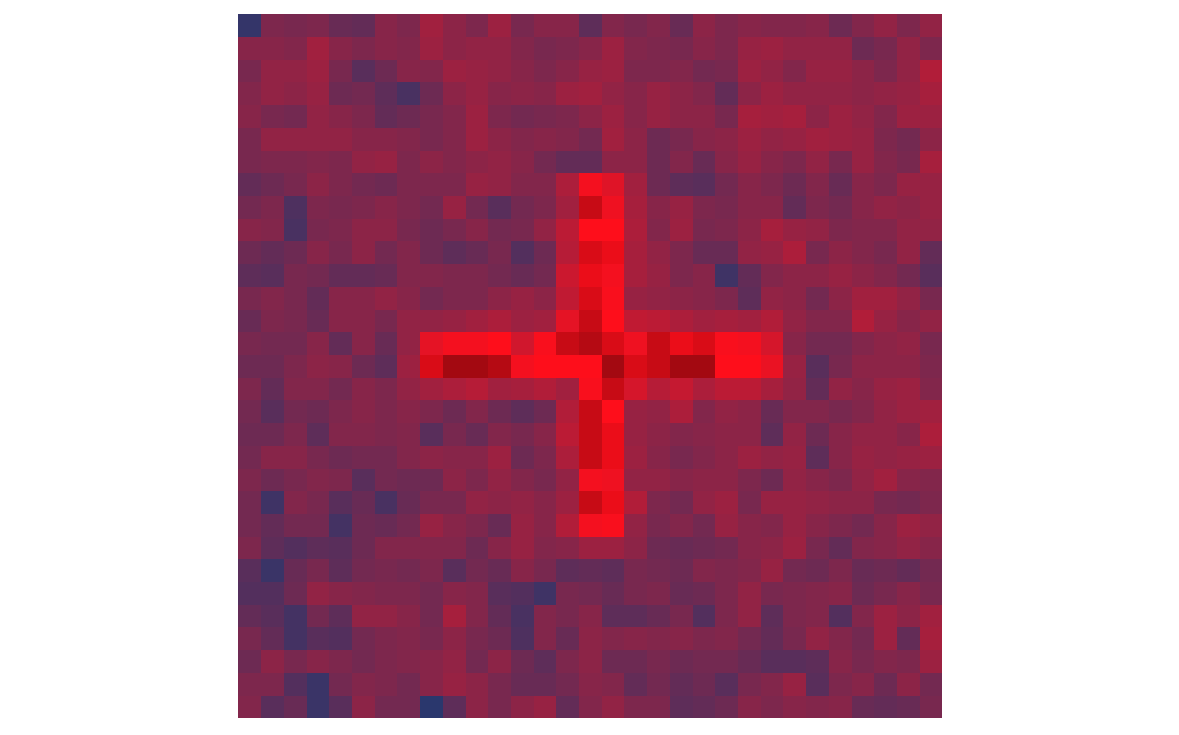
\includegraphics[width=1.2\linewidth]{../plots_tables_images/1d1dcrop_5_6.eps}
        % \caption{}
    \end{subfigure}
    % \hspace{-1.0in}
    \begin{subfigure}[b]{.3\linewidth}
        \centering
        \includegraphics[width=1.2\linewidth]{../plots_tables_images/1d1dcrop_5_9.eps}
        % \caption{}
    \end{subfigure}


    \begin{subfigure}[b]{.3\linewidth}
        \centering
        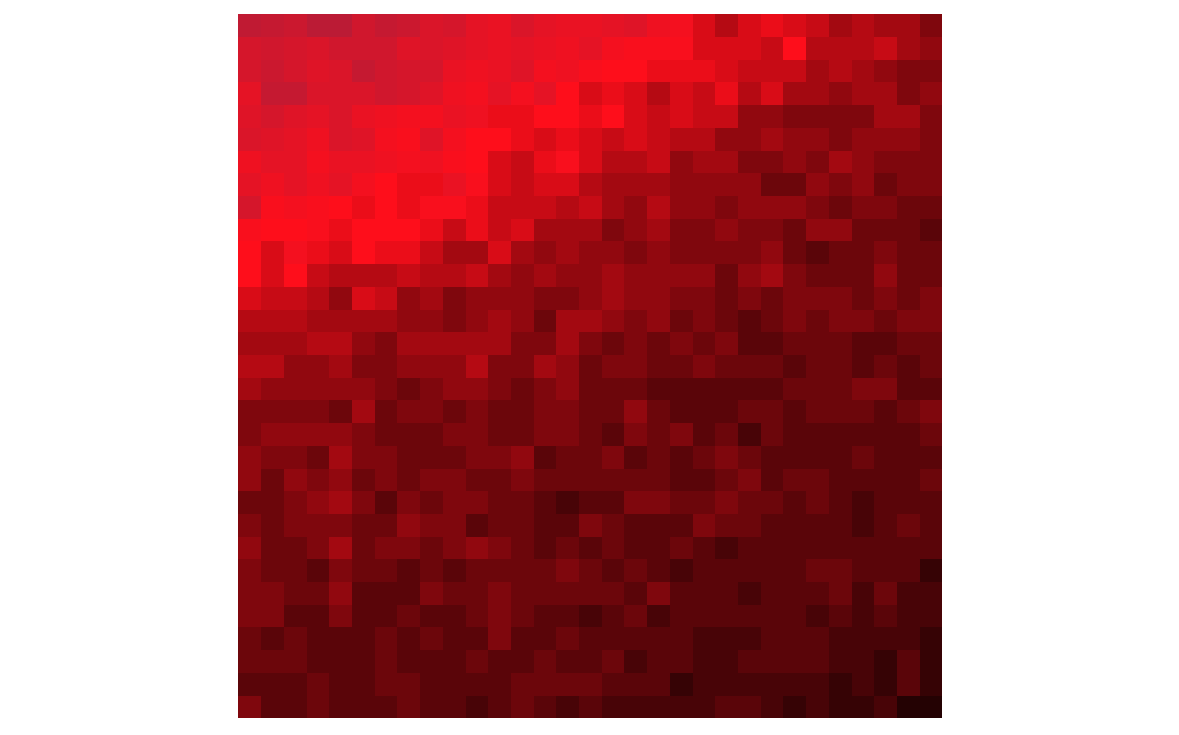
\includegraphics[width=1.2\linewidth]{../plots_tables_images/1d1dcrop_6_0.eps}
        % \caption{}
    \end{subfigure}
    % \hspace{-1.0in}
    \begin{subfigure}[b]{.3\linewidth}
        \centering
        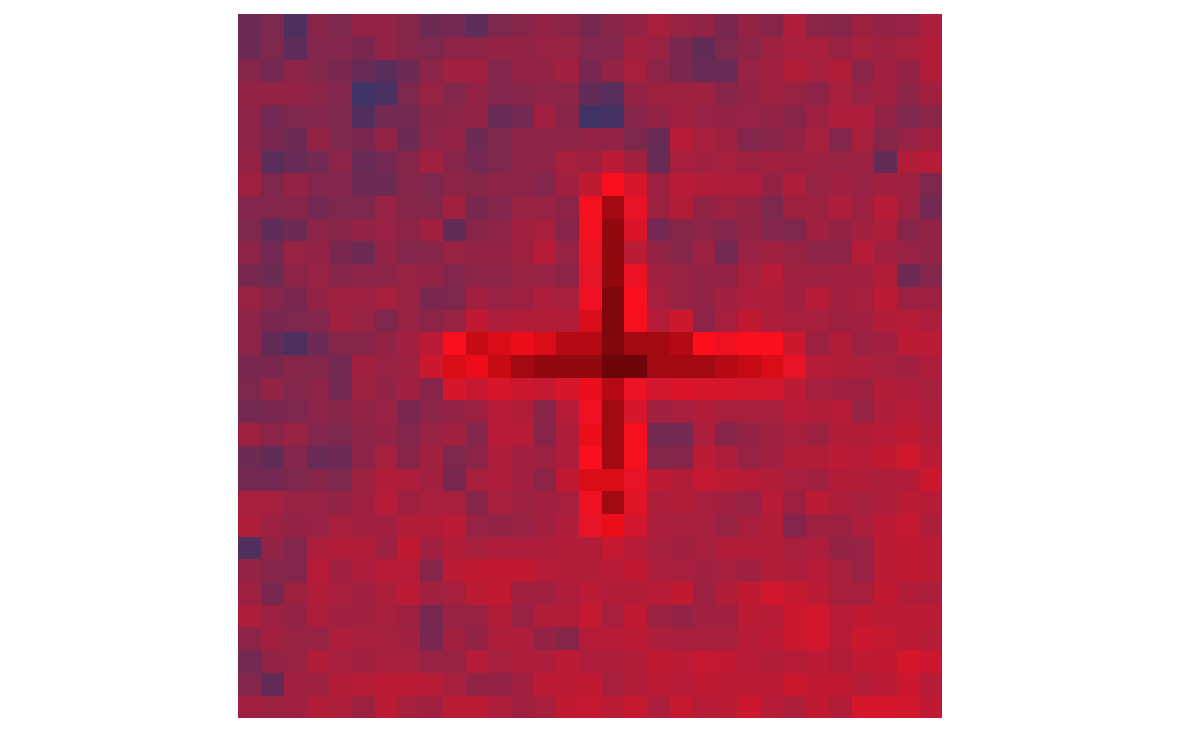
\includegraphics[width=1.2\linewidth]{../plots_tables_images/1d1dcrop_6_3.eps}
        % \caption{}
    \end{subfigure}
    \begin{subfigure}[b]{.3\linewidth}
        \centering
        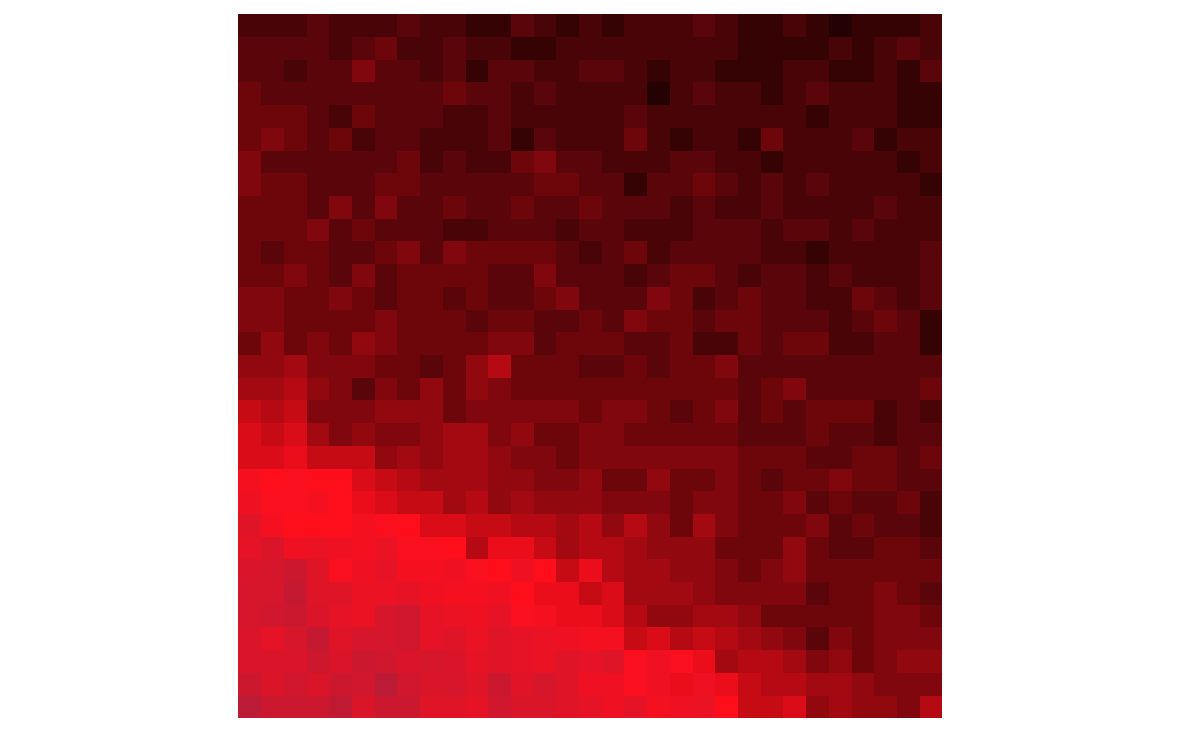
\includegraphics[width=1.2\linewidth]{../plots_tables_images/1d1dcrop_6_9.eps}
        % \caption{}
    \end{subfigure}
    \caption{Each possible fiducial candidate}
    \label{lotsofcrop}
\end{figure}


\begin{figure}[!ht]
    \vspace{-0.5in}
    \begin{subfigure}[b]{.3\linewidth}
        \centering
        \includegraphics[width=1.0\linewidth]{../plots_tables_images/1d1dsums_0_0.eps}
        % \caption{}
    \end{subfigure}
    \begin{subfigure}[b]{.3\linewidth}
        \centering
        \includegraphics[width=1.0\linewidth]{../plots_tables_images/1d1dsums_0_1.eps}
        % \caption{}
    \end{subfigure}
    % \hspace{-1.0in}
    \begin{subfigure}[b]{.3\linewidth}
        \centering
        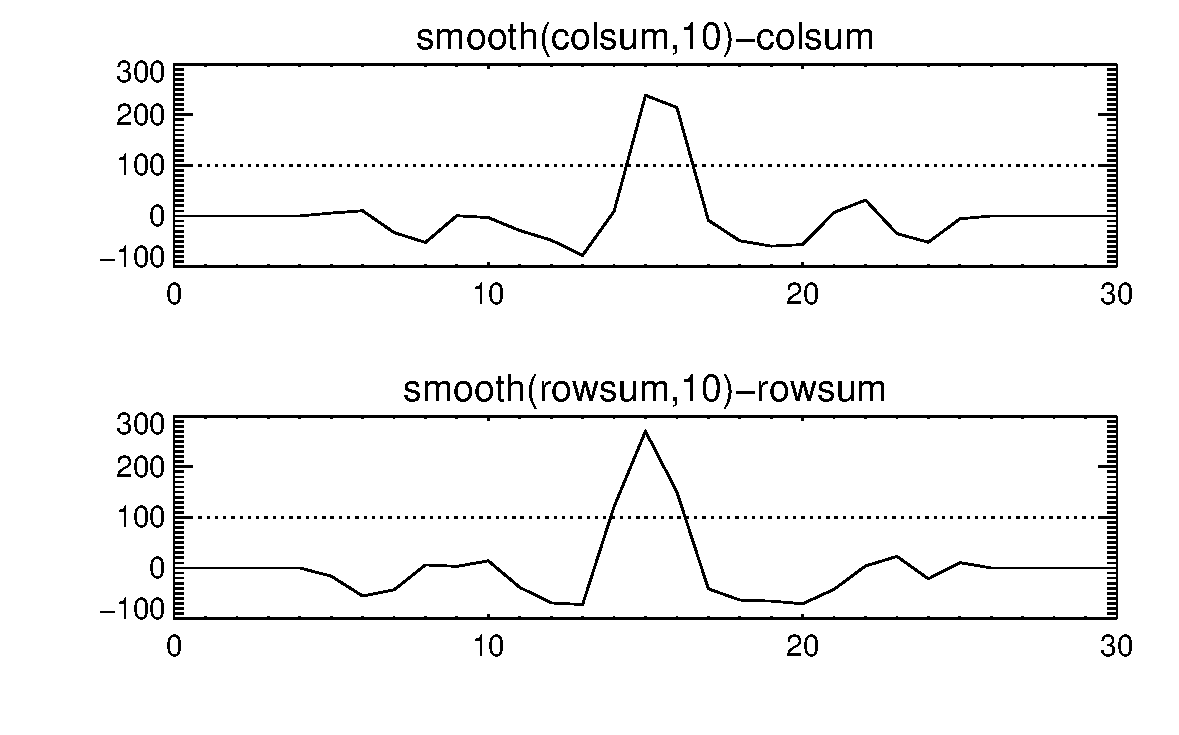
\includegraphics[width=1.0\linewidth]{../plots_tables_images/1d1dsums_0_4.eps}
        % \caption{}
    \end{subfigure}
\vspace{0.2in}

    \begin{subfigure}[b]{.3\linewidth}
        \centering
        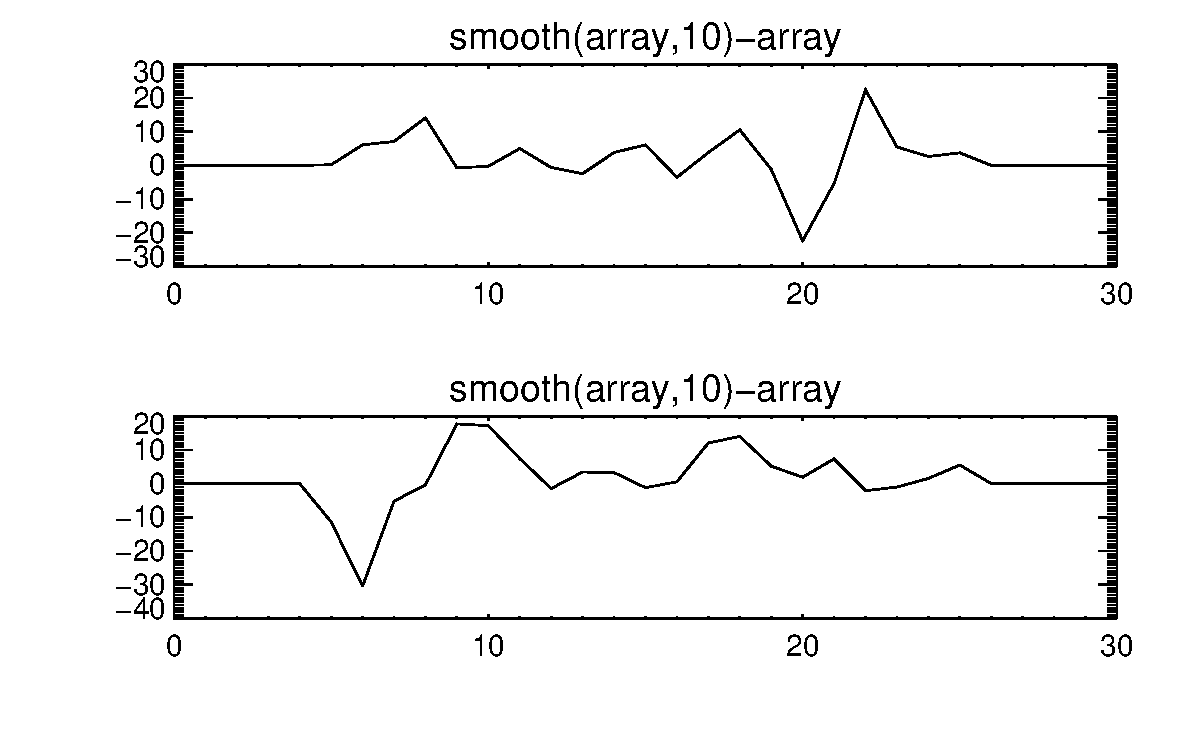
\includegraphics[width=1.0\linewidth]{../plots_tables_images/1d1dsums_0_8.eps}
        % \caption{}
    \end{subfigure}
    \begin{subfigure}[b]{.3\linewidth}
        \centering
        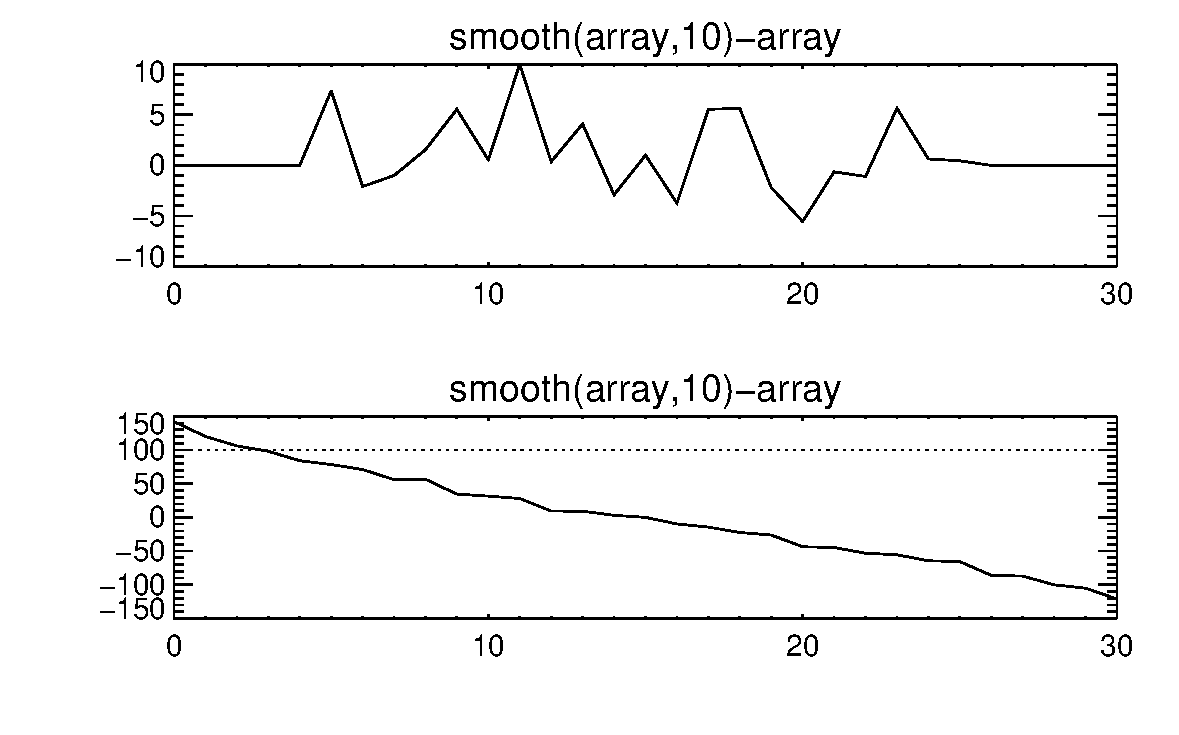
\includegraphics[width=1.0\linewidth]{../plots_tables_images/1d1dsums_0_9.eps}
        % \caption{}
    \end{subfigure}
    % \hspace{-1.0in}
    \begin{subfigure}[b]{.3\linewidth}
        \centering
        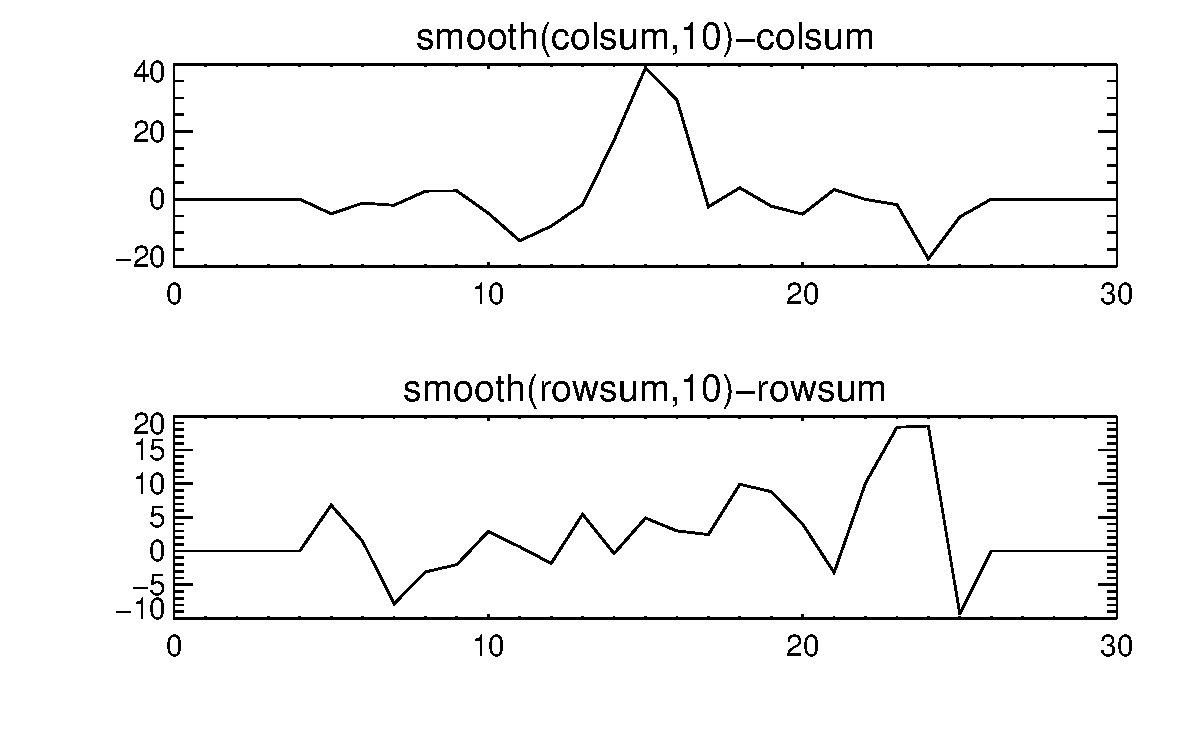
\includegraphics[width=1.0\linewidth]{../plots_tables_images/1d1dsums_1_0.eps}
        % \caption{}
    \end{subfigure}
\vspace{0.2in}

    \begin{subfigure}[b]{.3\linewidth}
        \centering
        \includegraphics[width=1.0\linewidth]{../plots_tables_images/1d1dsums_1_1.eps}
        % \caption{}
    \end{subfigure}
    \begin{subfigure}[b]{.3\linewidth}
        \centering
        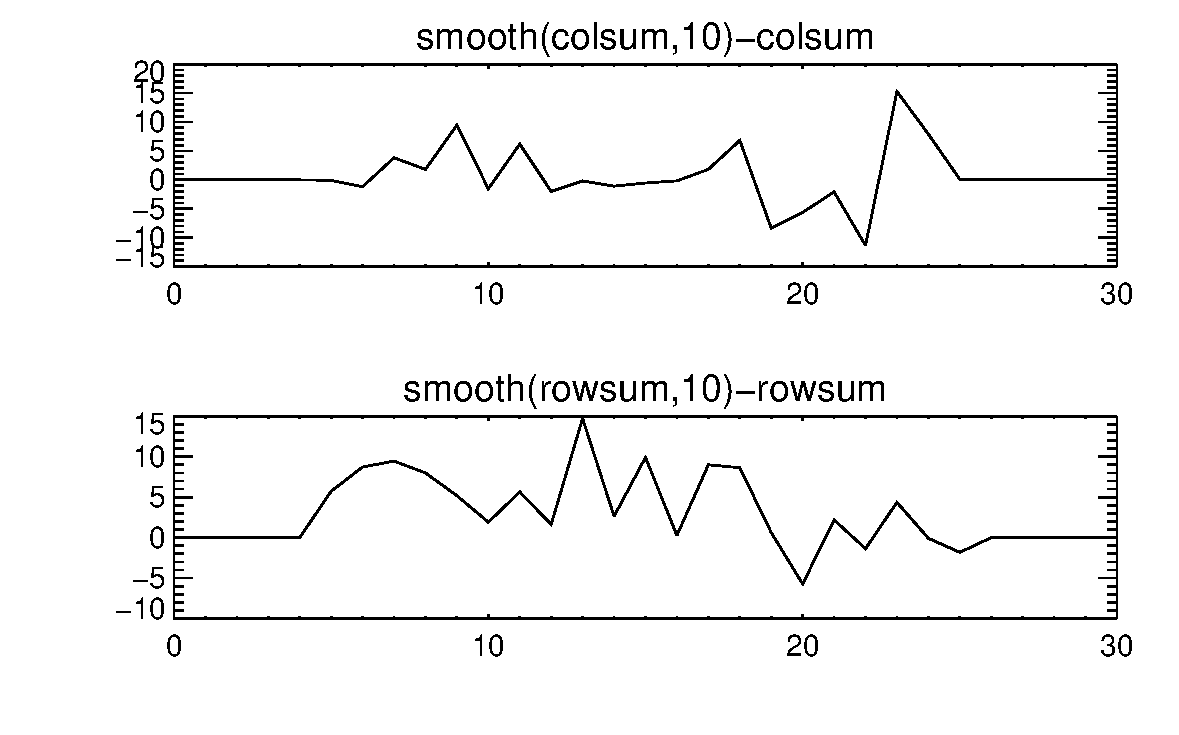
\includegraphics[width=1.0\linewidth]{../plots_tables_images/1d1dsums_1_9.eps}
        % \caption{}
    \end{subfigure}
    % \hspace{-1.0in}
    \begin{subfigure}[b]{.3\linewidth}
        \centering
        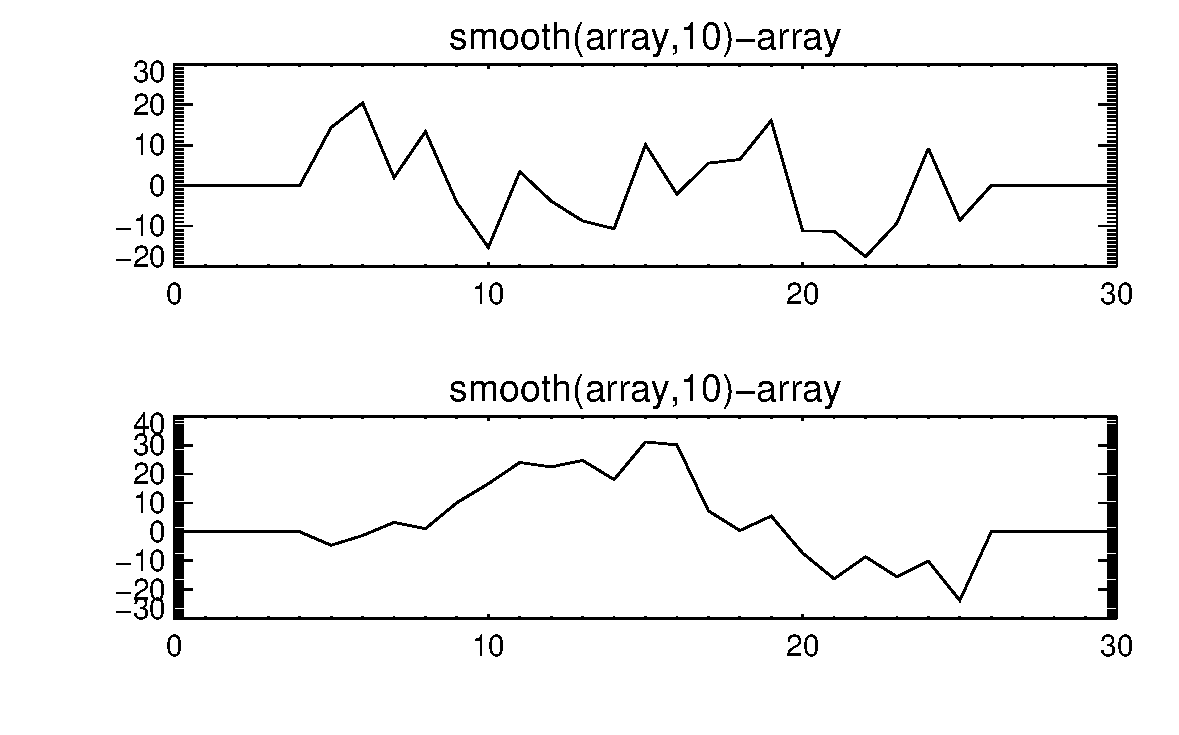
\includegraphics[width=1.0\linewidth]{../plots_tables_images/1d1dsums_2_0.eps}
        % \caption{}
    \end{subfigure}
\vspace{0.2in}

    \begin{subfigure}[b]{.3\linewidth}
        \centering
        \includegraphics[width=1.0\linewidth]{../plots_tables_images/1d1dsums_2_5.eps}
        % \caption{}
    \end{subfigure}
    \begin{subfigure}[b]{.3\linewidth}
        \centering
        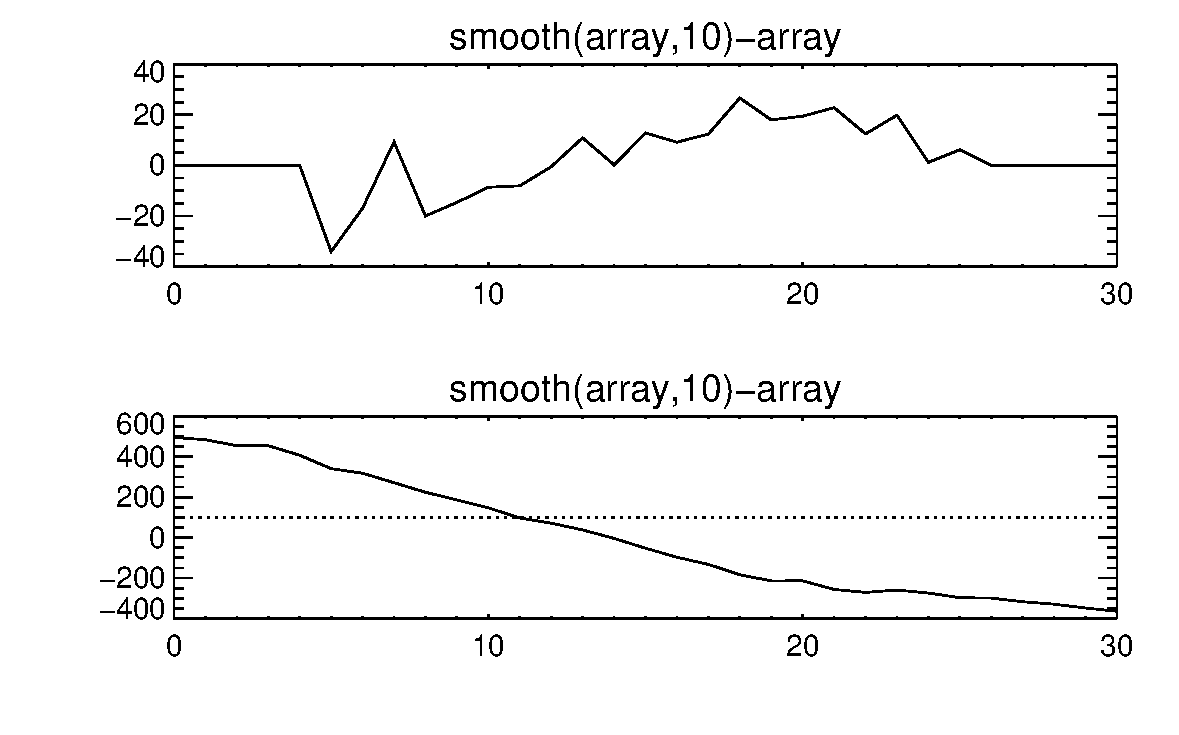
\includegraphics[width=1.0\linewidth]{../plots_tables_images/1d1dsums_2_9.eps}
        % \caption{}
    \end{subfigure}
    % \hspace{-1.0in}
    \begin{subfigure}[b]{.3\linewidth}
        \centering
        \includegraphics[width=1.0\linewidth]{../plots_tables_images/1d1dsums_3_0.eps}
        % \caption{}
    \end{subfigure}
\vspace{0.2in}

    \begin{subfigure}[b]{.3\linewidth}
        \centering
        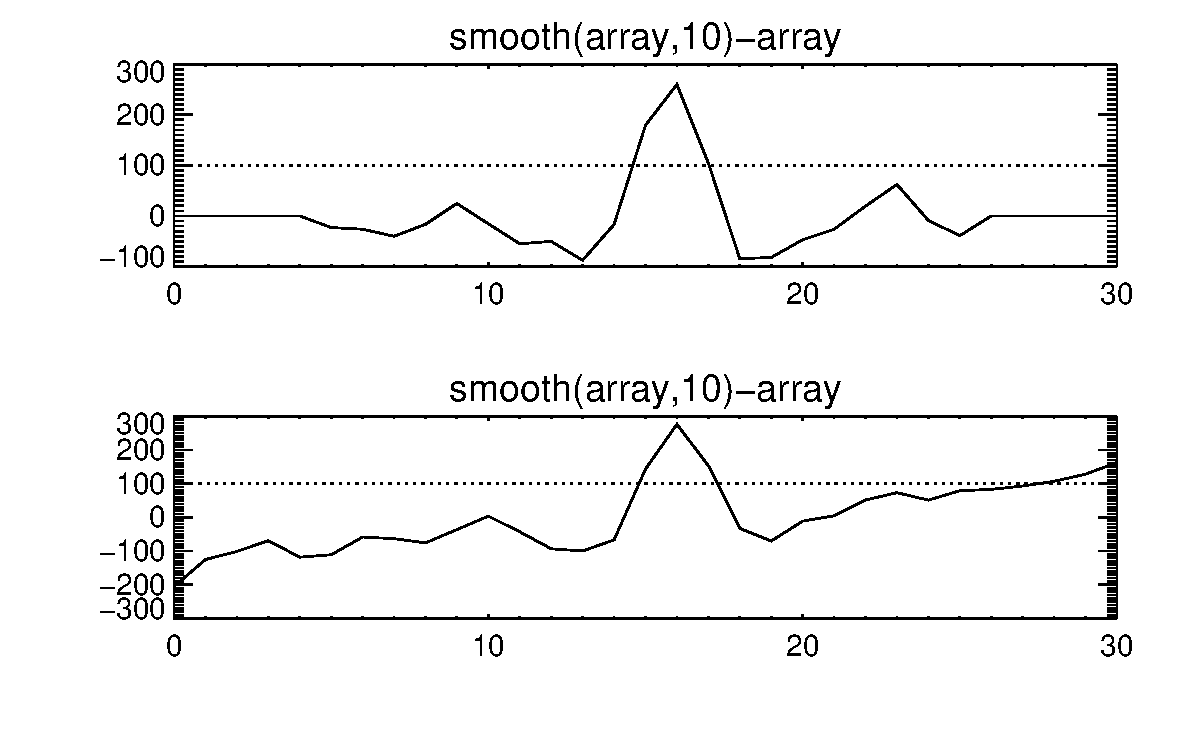
\includegraphics[width=1.0\linewidth]{../plots_tables_images/1d1dsums_3_2.eps}
        % \caption{}
    \end{subfigure}
    \begin{subfigure}[b]{.3\linewidth}
        \centering
        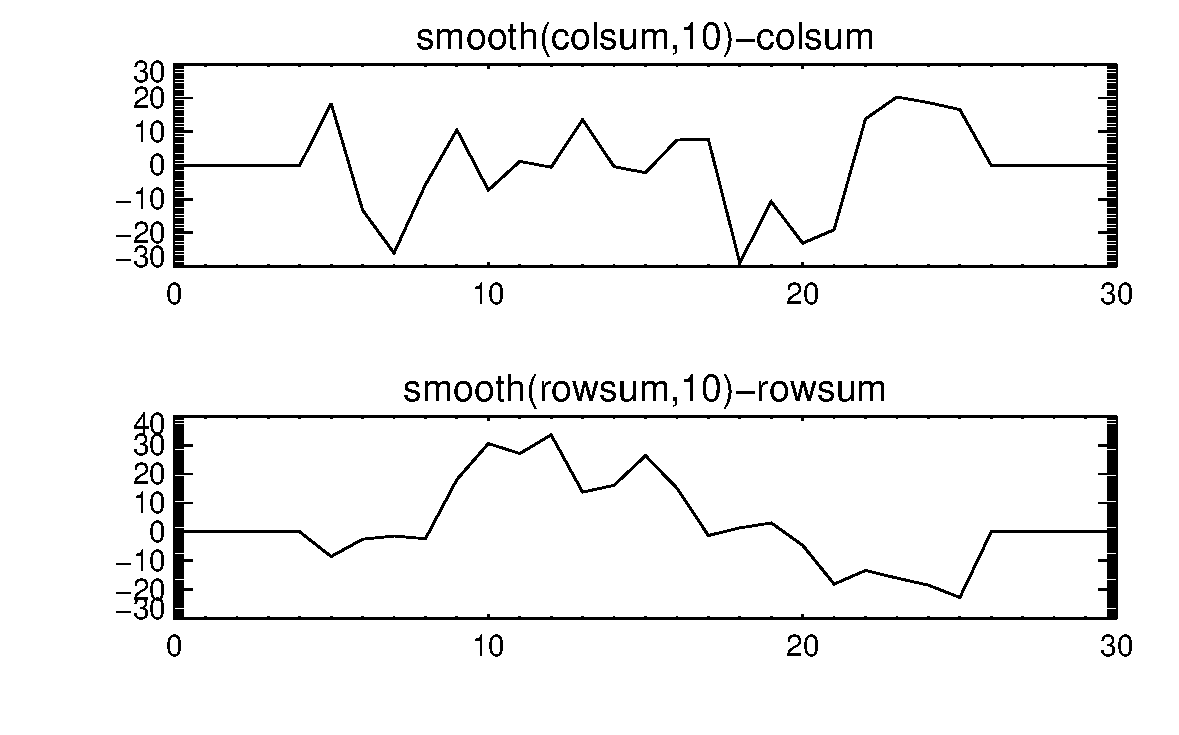
\includegraphics[width=1.0\linewidth]{../plots_tables_images/1d1dsums_4_0.eps}
        % \caption{}
    \end{subfigure}
    % \hspace{-1.0in}
    \begin{subfigure}[b]{.3\linewidth}
        \centering
        \includegraphics[width=1.0\linewidth]{../plots_tables_images/1d1dsums_4_9.eps}
        % \caption{}
    \end{subfigure}
\vspace{0.2in}

    \begin{subfigure}[b]{.3\linewidth}
        \centering
        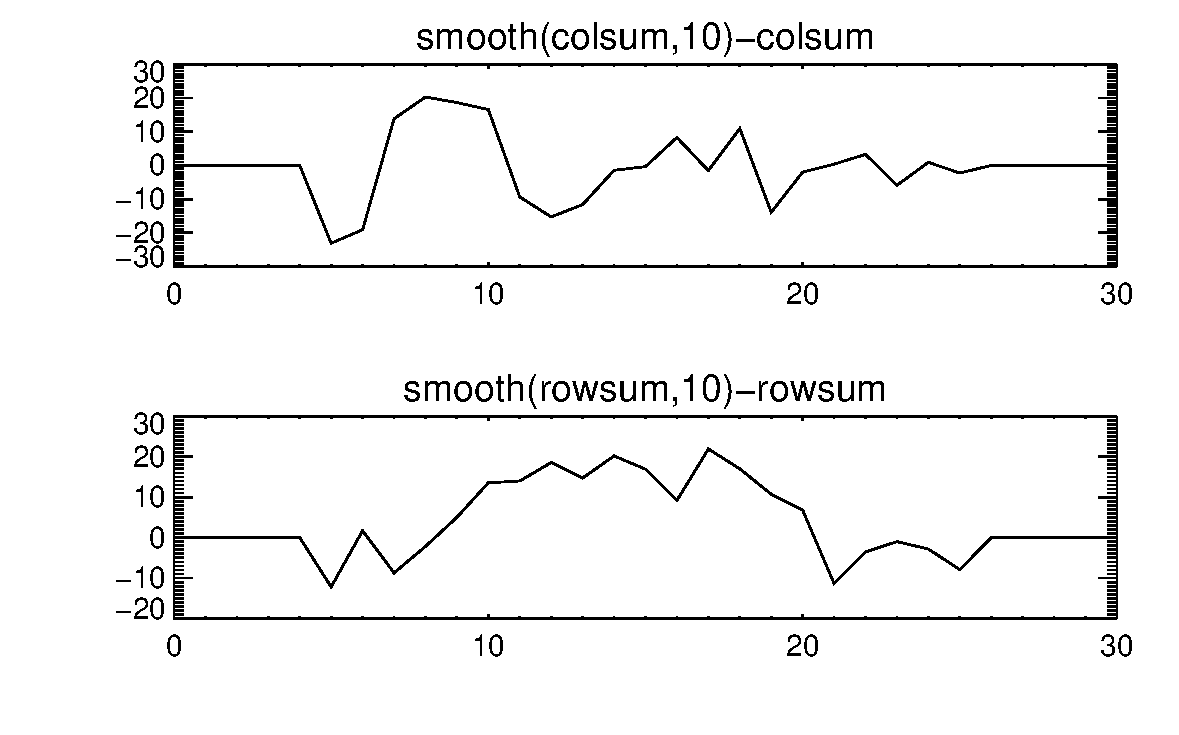
\includegraphics[width=1.0\linewidth]{../plots_tables_images/1d1dsums_5_0.eps}
        % \caption{}
    \end{subfigure}
    \begin{subfigure}[b]{.3\linewidth}
        \centering
        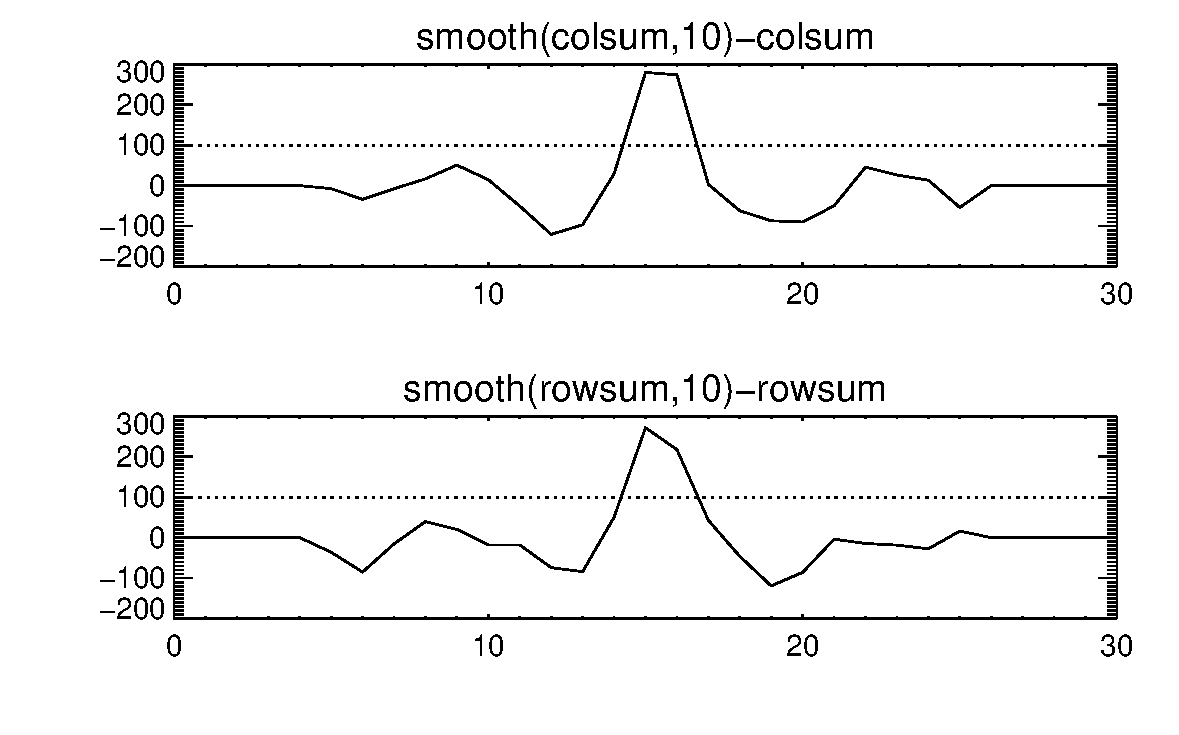
\includegraphics[width=1.0\linewidth]{../plots_tables_images/1d1dsums_5_6.eps}
        % \caption{}
    \end{subfigure}
    % \hspace{-1.0in}
    \begin{subfigure}[b]{.3\linewidth}
        \centering
        \includegraphics[width=1.0\linewidth]{../plots_tables_images/1d1dsums_5_9.eps}
        % \caption{}
    \end{subfigure}
\vspace{0.2in}

    \begin{subfigure}[b]{.3\linewidth}
        \centering
        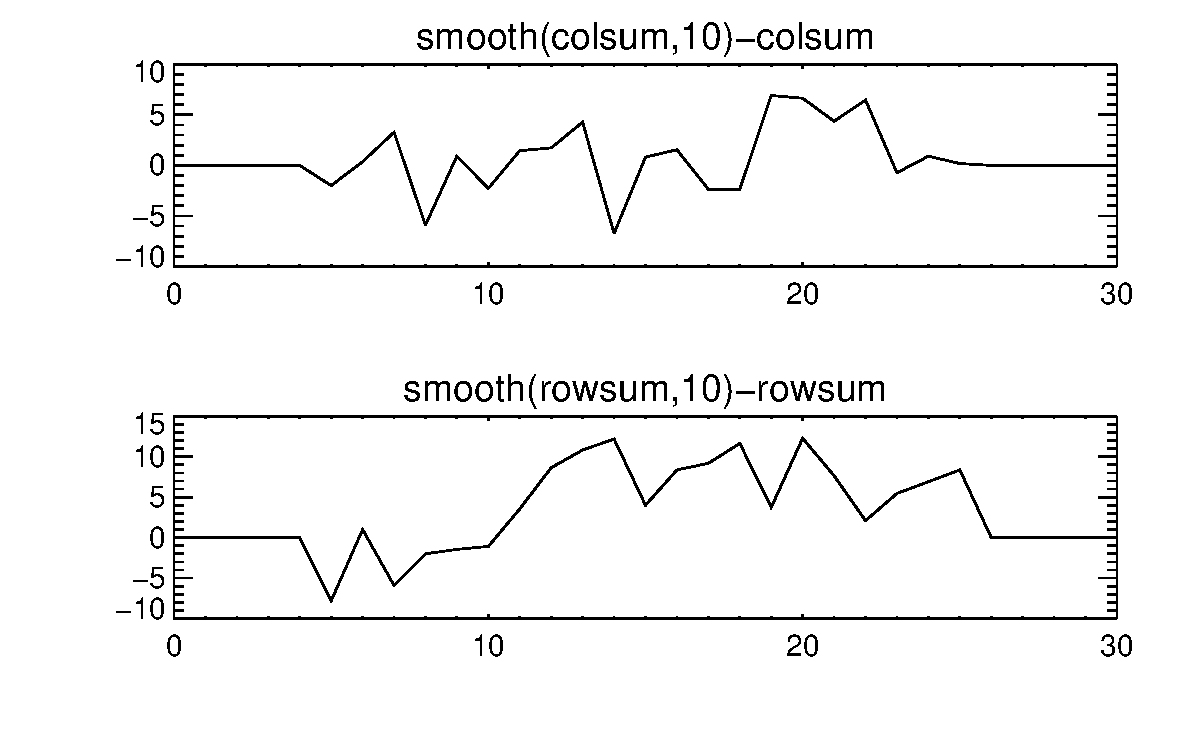
\includegraphics[width=1.0\linewidth]{../plots_tables_images/1d1dsums_6_0.eps}
        % \caption{}
    \end{subfigure}
    % \hspace{-1.0in}
    \begin{subfigure}[b]{.3\linewidth}
        \centering
        \includegraphics[width=1.0\linewidth]{../plots_tables_images/1d1dsums_6_3.eps}
        % \caption{}
    \end{subfigure}
    \begin{subfigure}[b]{.3\linewidth}
        \centering
        \includegraphics[width=1.0\linewidth]{../plots_tables_images/1d1dsums_6_9.eps}
        % \caption{}
    \end{subfigure}
    \caption{The horizontal line is at 100; if there are any elements of the array above 100 for both a column 1D sum and a row 1D sum, then the cropped area is identified to have a fiducial in it.}
    \label{lotsofplot}
\end{figure}

\subsection{Sub-Pixel Fitting} % (fold)
\label{sub:sub_pixel_fitting}
Once I know where the peaks are in the arrays of Figure \ref{lotsofplot}, I fit a parabola to the 3 pixels encompassing the peak maximum in each direction. 

% subsection sub_pixel_fitting (end)

% subsection 1d_sums (end)

% section finding_fiducials (end)


\section{Comparison of Fiducial Finding Methods} % (fold)
\label{sec:comparison_of_fiducial_finding_methods}

Table \ref{fidcomp} compares the Gaussian and parabolic-peak fitting results to Albert's fiducial positions.

\begin{deluxetable}{cccccccc}
\tablecaption{Comparison of peak-fitting}
\tabletypesize{\scriptsize}
\tablewidth{0pt}
\tablehead{
    \colhead{X pos} %
&   \colhead{Sub-pixel x} %
&   \colhead{Sub-pixel x} %
&   \colhead{Albert's x} %
&   \colhead{Y pos} %
&   \colhead{Sub-pixel y} %
&   \colhead{Sub-pixel y} %
&   \colhead{Albert's y}  \\

    \colhead{} %
&   \colhead{(Parabolic} %
&   \colhead{(Gaussian} %
&   \colhead{}
&   \colhead{}
&   \colhead{(Parabolic}
&   \colhead{(Gaussian} %
&   \colhead{} \\

    \colhead{} %
&   \colhead{Peak Fitting)} %
&   \colhead{Peak Fitting)} %
&   \colhead{}
&   \colhead{}
&   \colhead{Peak Fitting)} %
&   \colhead{Peak Fitting)} %
&   \colhead{}
}
\startdata
54  & 54.4053 & 54.4478 & 53.9459 & 108 & 107.946 & 108.044 & 109.100\\
70  & 70.3620 & 70.3049 &  & 39  & 38.7651 & 37.7765 & \\
101 & 101.355 & 101.287 & 100.782 & 123 & 124.465 & 123.740 & 124.789\\
116 & 117.014 & 117.017 & 116.529 & 54  & 55.1857 & 54.8310 & 55.6844\\
136 & 135.756 & 135.700 &  & 215 & 213.553 & 217.142 & \\
151 & 151.477 & 151.437 & 150.967 & 139 & 138.696 & 139.406 & 140.352\\
166 & 166.980 & 166.882 & 166.390 & 70  & 69.6979 & 70.3697 & 71.3244
\enddata
\label{fidcomp}
\end{deluxetable}

\begin{lstlisting}
>> help,*(bbb[0])
** Structure <260a348>, 2 tags, length=180, data length=178, refs=1:
   REG             INT              1
   FIDARR          STRUCT    -> FIDPOS Array[11]
>> help,(*(bbb[0])).fidarr,/str
** Structure FIDPOS, 4 tags, length=16, data length=16:
   X               FLOAT           50.0000
   Y               FLOAT           132.000
   SUBX            FLOAT           50.8438
   SUBY            FLOAT           133.291
\end{lstlisting}
% section comparison_of_fiducial_finding_methods (end)

\end{document}










